%\documentclass[a4paper,12pt]{report}
\documentclass[a4paper,12pt]{extreport}
 

%%% Поля и разметка страницы %%%
\usepackage{lscape}	    % Для включения альбомных страниц
\usepackage{geometry}	% Для последующего задания полей
%\usepackage{subfigure}  % Для создания рисунков с несколькими панелями

%%% Кодировки и шрифты %%%
\usepackage{cmap}			% Улучшенный поиск русских слов в полученном pdf-файле
\usepackage[T2A]{fontenc}		% Поддержка русских букв
\usepackage[utf8]{inputenc}		% Кодировка utf8
\usepackage[english, russian]{babel}	% Языки: русский, английский
%\usepackage{pscyr}			% Красивые русские шрифты
\usepackage{braket}

%%% Математические пакеты %%%
\usepackage{amsthm,amsfonts,amsmath,amssymb,amscd} % Математические дополнения от AMS

%%% Оформление абзацев %%%
\usepackage{indentfirst} % Красная строка

%%% Цвета %%%
\usepackage[usenames]{color}
\usepackage{color}
\usepackage{colortbl}

%%% Таблицы %%%                        
%\usepackage{longtable}			% Длинные таблицы
%\usepackage{multirow,makecell,array}	% Улучшенное форматирование таблиц

%%% Общее форматирование
\usepackage[singlelinecheck=off]{caption}	% Многострочные подписи
%\usepackage{soul}					% Поддержка переносоустойчивых подчёркиваний и зачёркиваний

%%% Библиография %%%
\usepackage[numbers]{natbib}
%\usepackage{cite} % Красивые ссылки на литературу
%\usepackage{csquotes}
%\usepackage[autolang=other,       
%            bibencoding=utf8,
%            sorting=none, % Name,Title,Year или sorting=none.
%            maxbibnames=3, % Максимальное число авторов в списке литературы.
%            minbibnames=2, % Число авторов, отображаемое при сокращении.
%            style=gost-numeric,
%            backend=biber]{biblatex}


\usepackage{placeins}

%%% Гиперссылки %%%
\usepackage[linktocpage=true,plainpages=false,pdfpagelabels=false,unicode=true]{hyperref}

%%% Изображения %%%
\usepackage{graphicx} % Подключаем пакет работы с графикой
%\usepackage{epstopdf}

%%% Оглавление %%%
\usepackage{tocloft}

\usepackage{titlesec}

%\usepackage{minted} %консольные комманды
\usepackage{listings}
\usepackage{tabularx} %растягивание колонок и перенос текста
\usepackage{xtab} %многостраничные таблицы
		% Подключаемые пакеты
%%% Макет страницы %%%
\geometry{a4paper,top=2cm,bottom=2cm,left=2cm,right=2cm}

\titleformat{\chapter}[display]
  {\normalfont\Large\filcenter\bfseries}{\chaptertitlename\ \thechapter}{20pt}{\LARGE}
\titlespacing*{\chapter}
  {0pt}{30pt}{20pt}

% см. http://tex.stackexchange.com/questions/134031/how-to-adjust-the-size-and-placement-of-chapter-heading-in-report-class
% и http://tex.stackexchange.com/questions/59726/change-size-of-section-subsection-subsubsection-paragraph-and-subparagraph-ti

%%% Кодировки и шрифты %%%
%\renewcommand{\rmdefault}{ftm} % Включаем Times New Roman

%%% Выравнивание и переносы %%%
\sloppy					% Избавляемся от переполнений
\clubpenalty=10000		% Запрещаем разрыв страницы после первой строки абзаца
\widowpenalty=10000		% Запрещаем разрыв страницы после последней строки абзаца
\linespread{1.3}

%%% Библиография %%%
\makeatletter
\bibliographystyle{ugost2008ns_v1.bst}	% Оформляем библиографию в соответствии с ГОСТ 7.0.5
%\bibliographystyle{utf8gost705u}
%\bibliographystyle{ugost2008}
\renewcommand{\@biblabel}[1]{#1.}	% Заменяем библиографию с квадратных скобок на точку:
\makeatother

%%% Изображения %%%
\graphicspath{{img_part1/}{img_part2/}{img_part3/}{img_part4/}{img_part5/}} % Пути к изображениям

%%% Цвета гиперссылок %%%
\definecolor{linkcolor}{rgb}{0.9,0,0}
\definecolor{citecolor}{rgb}{0,0,1}
\definecolor{urlcolor}{rgb}{0,0,1}
\hypersetup{
    colorlinks, linkcolor={linkcolor},
    citecolor={citecolor}, urlcolor={urlcolor}
}

%%% Оглавление %%%
\renewcommand{\cftchapdotsep}{\cftdotsep}


\newcommand{\kws}{\textit{KW}\ }
\newcommand{\rmn}[1]{{\mathrm{#1}}}
\newcommand\fdg{\mbox{$.\!\!^\circ$}}%
\newcommand\farcm{\mbox{$.\mkern-4mu^\prime$}}%
\newcommand\farcs{\mbox{$.\!\!^{\prime\prime}$}}%
\newcommand\nodata{ ~$\cdots$~ }%

			% Пользовательские стили

% journals

\def\apj{ApJ}
\def\apjl{ApJ Lett.}
\def\mnras{MNRAS}
\def\nat{Nature}
\def\physrevB{Phys. Rev. B}
\def\prd{Phys. Rev. D}
\def\prl{Phys. Rev. Lett.}
\def\pre{Phys. Rev. E}
\def\araa{Ann. Rev. Astron. Astrophys.}                % "Ann. Rev. Astron. Astrophys."
\def\aap{Astron. Astrophys.}                  % "Astron. Astrophys."
\def\aaps{Astron. Astrophys. Suppl. Ser.}                 % "Astron. Astrophys. Suppl. Ser."
\def\aj{Astron. J.}                      % "Astron. J."
\def\apjs{Astrophys. J. Suppl. Ser.}                  % "Astrophys. J. Suppl. Ser."
\def\pasp{Publ. Astron. Soc. Pac.}                  % "Publ. Astron. Soc. Pac."
\def\apjl{ApJ Lett.}                   % letter at ApJ
\def\pasj{PASJ}
\def\apss{Astroph. Space Sci.}
\def\aplett{Astroph. Lett.}
\def\ssr{Space Sci. Rev.}
\def\jcap{J. Cosmol. Astropart. Phys.}
\def\apspr{Sov. Sci. Rev. Sect. E}
\def\nar{New Astron. Rev.}
\def\aapr{ Astron. Astrophys. Rev.}

\begin{document}

%%% Переопределение именований %%%
\renewcommand{\abstractname}{Аннотация}
\renewcommand{\alsoname}{см. также}
\renewcommand{\appendixname}{Приложение}
\renewcommand{\bibname}{Литература}
\renewcommand{\ccname}{исх.}
\renewcommand{\chaptername}{Глава}
\renewcommand{\contentsname}{Содержание}
\renewcommand{\enclname}{вкл.}
\renewcommand{\figurename}{Рисунок}
\renewcommand{\headtoname}{вх.}
\renewcommand{\indexname}{Предметный указатель}
\renewcommand{\listfigurename}{Список рисунков}
\renewcommand{\listtablename}{Список таблиц}
\renewcommand{\pagename}{Стр.}
\renewcommand{\partname}{Часть}
\renewcommand{\refname}{Список литературы}
\renewcommand{\seename}{см.}
\renewcommand{\tablename}{Таблица}
			% Переопределение именований

\thispagestyle{empty}



\begin{center}
{\small
ФЕДЕРАЛЬНОЕ ГОСУДАРСТВЕННОЕ БЮДЖЕТНОЕ УЧРЕЖДЕНИЕ НАУКИ\\
ФИЗИКО-ТЕХНИЧЕСКИЙ ИНСТИТУТ ИМ.~А.Ф.~ИОФФЕ РОССИЙСКОЙ АКАДЕМИИ НАУК\\
}
\end{center}

\begin{figure}
	\centering
	
\includegraphics[width=5.5 cm]{./fig/ioffe.png} 
\end{figure}



\vspace{5mm}
\begin{center}
{\bf \Huge FAINA
\par}
\vspace{10mm}
%Astrophysical code for modeling radiation sources 
Астрофизический код для моделирования наблюдаемых потоков от источников излучения
\vspace{10mm}
%User's guide
{\bf \large Руководство пользователя \par}
\end{center}




\vspace{120mm}
\begin{center}
{Санкт-Петербург~--- 2023}
\end{center}

\newpage			% Титульный лист
\tableofcontents
\clearpage
		% Оглавление
\chapter*{Введение}		
\addcontentsline{toc}{chapter}{Введение}	%добавляем в оглавление			
FAINA - численный код, предназначенный для расчетов различных видов электромагнитного излучения от астрофизических источников. Код написан на языке C++ с использованием только стандартной библиотеки. В текущей версии кода реализованы следующие виды излучения: синхротронное излучение, излучение за счет обратного комптоновского рассеяния, излучение распада пионов в результате свободно-свободных столкновений протонов, а так же тормозное излучение. FAINA позволяет вычислять наблюдаемые потоки от источников с заданными параметрами, а так же вычислять параметры источников с помощью фитирования наблюдаемых данных расчетными. Так же возможен учет эволюции источников и их излучения во времени.

\section*{Установка и запуск}
\addcontentsline{toc}{section}{Установка и запуск}
Текущая версия кода доступна на github https://github.com/VadimRomansky/Faina. Скачайте архив и разархивируйте его в директорию Faina.
\subsection*{Windows}
\addcontentsline{toc}{subsection}{Windows}
Для работы с кодом и его запуска в операционной системе Windows необходимо использовать Microsoft Visual Studio и открыть с помощью неё файл Faina.sin, содержащийся в корневой директории кода. Работоспособность проверялась на версии Visual Studio 2022.
\subsection*{Linux}
\addcontentsline{toc}{subsection}{Linux}
Для запуска FAINA в операционной системе Linux предусмотрены два варианта. Рекомендуется использовать среду разработки QtCreator и открыть с помощью неё проектный файл Faina.pro, содержащийся в корневой дирректории кода. 

Так же возможна непосредственная компиляция и запуск из терминала, с помощью комманд
\begin{lstlisting}[language=bash]
	$ g++ -o faina *.cpp
	$ ./faina
\end{lstlisting}
\section*{Быстрый старт}\label{quickStart}
\addcontentsline{toc}{section}{Быстрый старт}
Рассмотрим простейший пример, приведенный в процедуре evaluateSimpleSynchrotron в файле main.cpp. В данном примере рассмытривается синхротронное излучение от однородного источника в форме плоского диска, с заданной степенной функцией распределения излучающих электронов. Сначала зададим значения магнитного поля и концентрации электронов (в коде используются единицы СГС).

\begin{lstlisting}[language=c++]
	double B = 1.0;
	double electronConcentration = 1.0;
\end{lstlisting}

После этого нужно создать распределение электронов. Вычисление синхротрона реализовано только для изотропного распределения, поэтому создадим изотропное степенное распределение. Конструктор степенного распределения принимает следующие параметры: массу частиц, подставим константу - массу электрона, степенной индекс (он считается положительным и должен быть больше 1), энергию, с которой начинается спектр, в качестве нее выберем энергию покоя электронов, и концентрацию электронов.

\begin{lstlisting}[language=c++]
	MassiveParticleIsotropicDistribution* distribution =
	new MassiveParticlePowerLawDistribution(
	massElectron, 3.0, me_c2, electronConcentration);
\end{lstlisting}

Далее создадим источник излучения - однородный плоский диск, парметры его конструктора это распределение электронов, магнитное поле, синус угла наклона магнитного поля к лучу зрения, радиус, толщина и расстояние до него.

\begin{lstlisting}[language=c++]
	RadiationSource* source = new SimpleFlatSource(
	distribution, B, 1.0, parsec, parsec, 1000 * parsec);
\end{lstlisting}

Последнее, что нам нужно - вычислитель потока излучения. Ему нужно указать рассматриваемый диапазон энергий электронов, в виде числа точек разбиения для интегрирования, минимальной и максимальной энергии. Так же есть параметр, отвечающий за учет синхротронного самопоглощения, по умолчанию его значение true.

\begin{lstlisting}[language=c++]
	RadiationEvaluator* evaluator = new 
	SynchrotronEvaluator(1000, me_c2, 1000 * me_c2, true);
\end{lstlisting}

Синхротронное приближение применимо только при частотах, намного больших циклотронной, поэтому вычислим её

\begin{lstlisting}[language=c++]
	double cyclOmega = 
	electron_charge * B / (massElectron * speed_of_light);
\end{lstlisting}

Теперь осталось только вычислить само излучение. У класса RadiationEvaluator есть метод, вычисляющий поток излучения в заданном диапазоне энергий и записывающий его в файл. Нужно указать имя файла, источник излучения, минимальную и максимальную энергии фотонов, и желаемое количество точек в этом диапазоне. Вычисление потока и вывод происходит в единицах энергия фотонов - энергетическая плотность потока излучения $\text{Вт}/ \text{эрг } {\text{см}}^2 = {\text{см}}^{-2} {\text{c}}^{-1}$. Если необходим вывод в других единицах, то запись в файл нужно переписать самостоятельно. 

\begin{lstlisting}[language=c++]
	evaluator->writeFluxFromSourceToFile("out.dat",source, 
	10*hplank*cyclOmega, 1E5*hplank*cyclOmega, 1000);
\end{lstlisting}


Функция вычисления синхротронного потока источника готова, осталось лишь вызвать её из основной процедуры main(). В результате вычисления должен получиться спектр источника, показанный на рисунке \ref{example0}
\begin{figure}
	\centering
	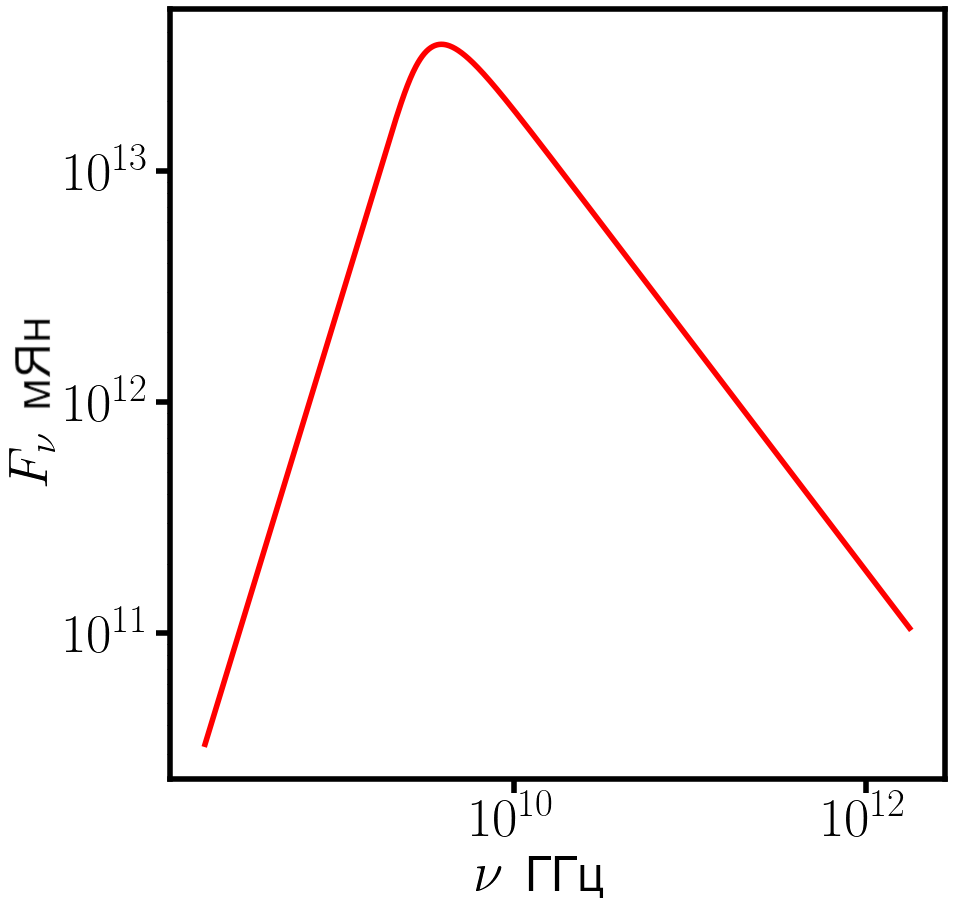
\includegraphics[width=12.5 cm]{./fig/example0.png} 
	\caption{Энергетическая плотность потока синхротронного излучения от тестового источника}
	\label{example0}
\end{figure}	% Введение
%\chapter{Расчет излучения источников}\label{radiation}
FAINA позволяет рассчитывать электромагнитное излучение от источников с заданными функциями распределения излучающих частиц и другими параметрами. Построены модели следующих типов излучения: синхротронного, обратного комптоновского рассеяния, пионного распада в результате свободно-свободного взаимодействия протонов и тормозного излучения.

\section{Функции распределения частиц}

Важнейшими исходными данными для расчета любого типа излучения является функция распределения излучающих частиц. В коде FAINA для представления распределений используется абстрактный класс ParticleDistribution и семейство наседованных от него классов, соответствующих различным конкретным реализациям. Класс ParticleDistribution имеет следующие доступные методы, описанные в Таблице \ref{ParticleDistribution}:

	\begin{table}
	\begin{center}
		\caption{Публичные методы класса ParticleDistribution }
		\label{ParticleDistribution}
		\begin{small}
		\begin{tabularx}{\textwidth}{|X|X|}
			\hline
			\textbf{ParticleDistribution} & Абстрактный класс для любых распределений частиц\\
			\hline
			distribution(const double\& energy, const double\& mu, const double\& phi) & возвращает функцию распределения от энергии, косинуса полярного угла и азимутального угла, нормированную на единицу \\
			\hline
			virtual distributionNormalized(const double\& energy, const double\& mu, const double\& phi) & чисто виртуальный метод, возвращает функцию распределения от энергии, косинуса полярного угла и азимутального угла, нормированную на концентрацию \\
			\hline
			getConcentration() & возвращает концентрацию частиц\\
			\hline
		\end{tabularx}
	    \end{small}
	\end{center}
\end{table}

Для вычисления излучения необходимо в первую очередь задать распределение излучающих частиц. Для это нужно создать объект из подходящего класса-наследника ParticleDistribution. Дерево наследования на две большие ветви - распределения фотонов, представленных абстрактным классом PhotonDistribution и распределения массивных частиц - MassiveParticleDistribution. Схема наследования этих классов представлена на рисунке \ref{particleDistribution0}. 

\begin{figure}
	\centering
	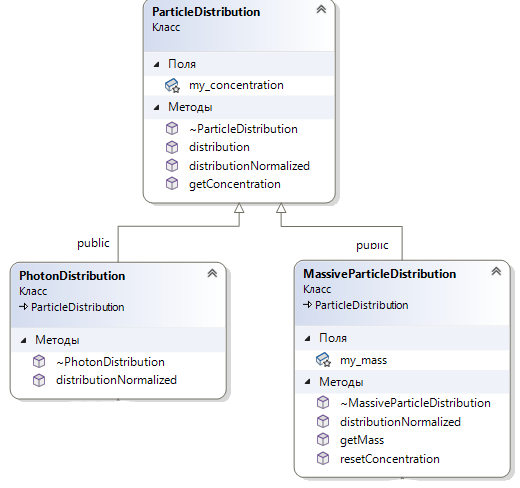
\includegraphics[width=9.5 cm]{./fig/particleDistribution0.png} 
	\caption{Схема наследования распределения фотонов и массивных частиц}
	\label{particleDistribution0}
\end{figure}

Важно отметить, что распределения фотонов не используются для представления результатов расчета излучения. Они нужны как входной параметр для расчета обратного комптоновского рассеяния. Класс PhotonDistribution не имеет дополнительных собственных методов и является лишь интерфейсом. Класс MassiveParticleDistribution тоже является абстрактным, в нем не задан конкретный вид распределения, но добавлены новые методы, описанные в Таблице \ref{MassiveParticleDistribution}	
\begin{table}
	\begin{center}
		\caption{Публичные методы класса MassiveParticleDistribution }
		\label{MassiveParticleDistribution}
		\begin{small}
			\begin{tabularx}{\textwidth}{|X|X|}
				\hline
				\textbf{MassiveParticleDistribution} & Абстрактный класс для распределений массивных излучающих частиц\\
				\hline
				getMass() & возвращает массу частиц \\
				\hline
				resetConcentration(const double\& n) & позволяет изменить полную концентрацию частиц в распределении\\
				\hline
			\end{tabularx}
		\end{small}
	\end{center}
\end{table}
\subsection{Распределения фотонов}

От абстрактного класса PhotonDistribution наследуются следующие классы: абстрактный PhotonIsotropicDistribution, предназначенный для представления изотропных распределений фотонов и CompoundPhotonDistribution, представляющий из себя сумму нескольких распределений фотонов общего вида. Схема наследования классов фотонных распределений представлена на рисунке \ref{photonDistribution}.

\begin{figure}
	\centering
	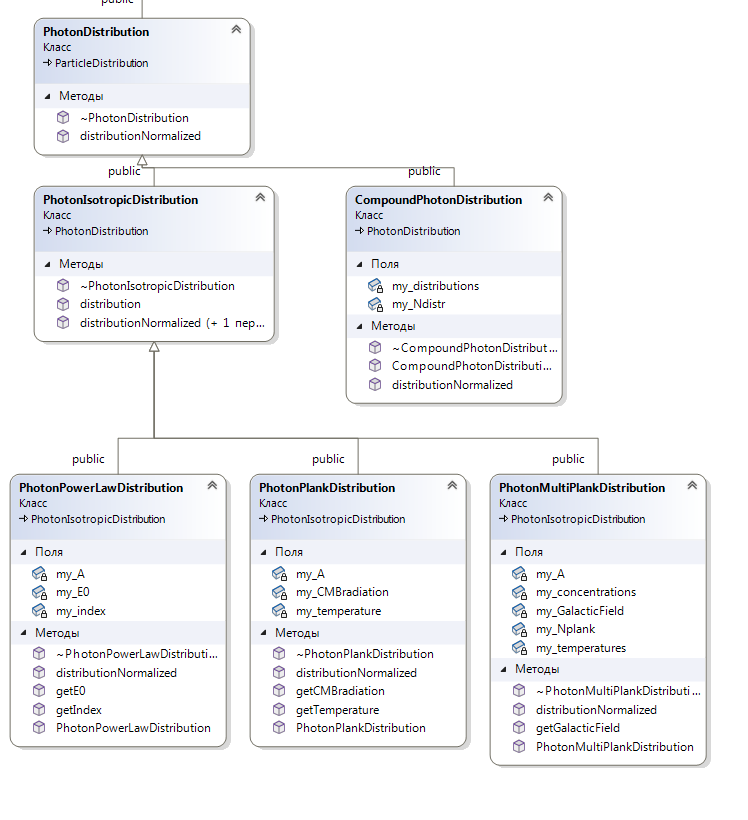
\includegraphics[width=10.5 cm]{./fig/photonDistribution1.png} 
	\caption{Схема наследования классов распределений фотонов}
	\label{photonDistribution}
\end{figure}

У изотропного распределения PhotonIsotropicDistribution добавляются методы, возвращающие значение функции распределения только в зависимости от энергии. Важно понимать, что это не функция распределения по энергии, а полная функция распределения с отброшенными угловыми аргументами. Другими словами, для получения значения функции распределения по энергии нужно домножить значение, возвращенное данным методом на $4 \pi$.

У класса PhotonIsotropicDistribution есть три наследника, которые уже не абстрактные классы, а непосредственно предназначены для создания распределений. Это PhotonPowerLawDistribution для представления степенных распределений, PhotonPlankDistribution, для планковских распределений и PhotonMultiPlankDistribution, для суммы планковских распределений. Метода класса PhotonIsotropicDistribution и его наследников перечислены в таблице \ref{photonDistributionMethods}

\begin{table}
	\begin{center}
		\caption{Публичные методы классов изотропных распределений фотонов}
		\label{photonDistributionMethods}
		\begin{small}
			\begin{tabularx}{\textwidth}{|X|X|}
				\hline
				\textbf{PhotonIsotropicDistribution} & Абстрактный класс для изотропных распределений фотонов\\
				\hline
				distribution(const double\& energy) & возвращает функцию распределения с отброшенными угловыми аргументами, то есть нормированную на концентрацию, деленную на $4 \pi$ \\
				\hline
				virtual distributionNormalized(const double\& energy) & чисто виртуальный метод, возвращает функцию распределения с отброшенными угловыми аргументами, нормированную на  $ 1 / 4 \pi$\\
				\hline
				\textbf{PhotonPowerLawDistribution} & Класс для степенного распределения фотонов\\
				\hline
				PhotonPowerLawDistribution(const double\& index, const double\& E0, const double\& concentration) & конструктор, создающий экземпляр с заданными показателем наклона, начальной энергией и полной концентрацией \\
				\hline
				getIndex() & возвращает показатель наклона спектра\\
				\hline
				getE0() & возвращает минимальную энергию степенного распределения\\
				\hline
				\textbf{PhotonPlankDistribution} & Класс для планковского распределения фотонов\\
				\hline
				PhotonPlankDistribution(const double\& temperature, const double\& amplitude) & конструктор, создающий экземпляр с заданными температурой и апмплитудой - то есть отношением концентрации к равновесному планковскому распределению с данной температурой\\
				\hline
				static getCMBRadiation() & статический метод, возвращающий экземпляр, соответствующий реликтовому излучению (температура $2.725 K$, амплитуда $1$)\\
				\hline
				getTemperature() & возвращает температуру распределения\\
				\hline
				\textbf{PhotonMultiPlankDistribution} & Класс для распределения фотонов, состоящего из суммы планковских распределений\\
				\hline
				PhotonMultiPlankDistribution(int Nplank, const double* const temperatures, const double* const amplitudes) & конструктор, количество планковских распределений, участвующих в смеси, массив их температур и массив амплитуд\\
				\hline
				static getGalacticField() & статический метод, возвращающий экземпляр, соответствующий среднегалактическому фотонному распределению, по данным статьи \cite{Mathis1983}. Данное распределение состоит из пяти планковских компонент, с температурами $2.725K, 20K, 3000K, 4000K, 7000K$ и амплитудами $1.0, 4\cdot10^{4}, 4\cdot10^{-13}, 1.65\cdot10^{-13}, 1.0\cdot10^{-14}$ соответственно\\
				\hline
			\end{tabularx}
		\end{small}
	\end{center}
\end{table}

Класс CompoundPhotonDistribution предназначен для представления смеси различных распределений фотонов, не обязательно планковских, как PhotonMultiPlankDistribution, и не обязательно изотропных. Его методы описаны в Таблице \ref{CompoundPhotonMethods}

\begin{table}
	\begin{center}
		\caption{Публичные методы класса CompoundPhotonDistribution }
		\label{CompoundPhotonMethods}
		\begin{small}
			\begin{tabularx}{\textwidth}{|X|X|}
				\hline
				\textbf{CompoundPhotonDistribution} & Класс для распределения фотонов, состоящего из суммы других распределений\\
				\hline
				CompoundPhotonDistribution(int N, PhotonDistribution** distributions) & конструктор, создающий экземпляр с заданным количеством распределений в смеси и массивом этих распределений \\
				\hline
				CompoundPhotonDistribution( PhotonDistribution* dist1, PhotonDistribution* dist2) & конструктор, создающий экземпляр содержащий смесь из двух распределений\\
				\hline
				CompoundPhotonDistribution( PhotonDistribution* dist1, PhotonDistribution* dist2, PhotonDistribution* dist3) & конструкторб создающий экземпляр содержащий смесь из трех распределений\\
				\hline
			\end{tabularx}
		\end{small}
	\end{center}
\end{table}

Встроенных анизотропных распределений фотонов в коде на данный момент нет, но пользователь может реализовать их самостоятельно, создав класс, наследующий от PhotonDistribution и определив необходимый виртуальный метод distributionNormalized(const double\& energy, const double\& mu, const double\& phi). Аналогично можно, конечно, создать и другие виды изотропных распределений.

\subsection{Распределения массивных частиц}
Распределения массивных частиц представлены наследниками класса MassiveParticleDistribution. Так же как и в случае с фотонами важную роль играет абстрактный клас для представления изотропных распределений - MassiveParticleIsotropicDistribution. У этого класса есть методы возвращающие значение функции распределения в зависимости от энергии, и опять же, это не функция распределения, проинтегрированная по углам, а полная функция распределения с отброшенными угловыми аргументами. Для получения значения функции распределения по энергии нужно домножить значение, возвращенное данным методом на $4 \pi$. Так же добавлен метод записи функции распределения в файл. 

\begin{table}
	\begin{center}
		\caption{Публичные методы класса MassiveParticleIsotropicDistribution }
		\label{MassiveParticleMethods}
		\begin{small}
			\begin{tabularx}{\textwidth}{|X|X|}
				\hline
				\textbf{MassiveParticleIsotropicDistribution} & Абстрактный класс для изотропных распределений\\
				\hline
				distribution(const double\& energy) & возвращает функцию распределения с отброшенными угловыми аргументами, то есть нормированную на концентрацию, деленную на $4 \pi$ \\
				\hline
				virtual distributionNormalized(const double\& energy) & чисто виртуальный метод, возвращает функцию распределения с отброшенными угловыми аргументами, нормированную на  $ 1 / 4 \pi$\\
				\hline
				writeDistribution(const char* fileName, int Ne, const double\& Emin, const double\& Emax) & записывает распределение в файл с данным именем, в диапазоне межджу данными минимальной и максимальной енергиями с заданным количеством точек, которые распределяются логарифмически\\
				\hline
			\end{tabularx}
		\end{small}
	\end{center}
\end{table}

\begin{figure}
	\centering
	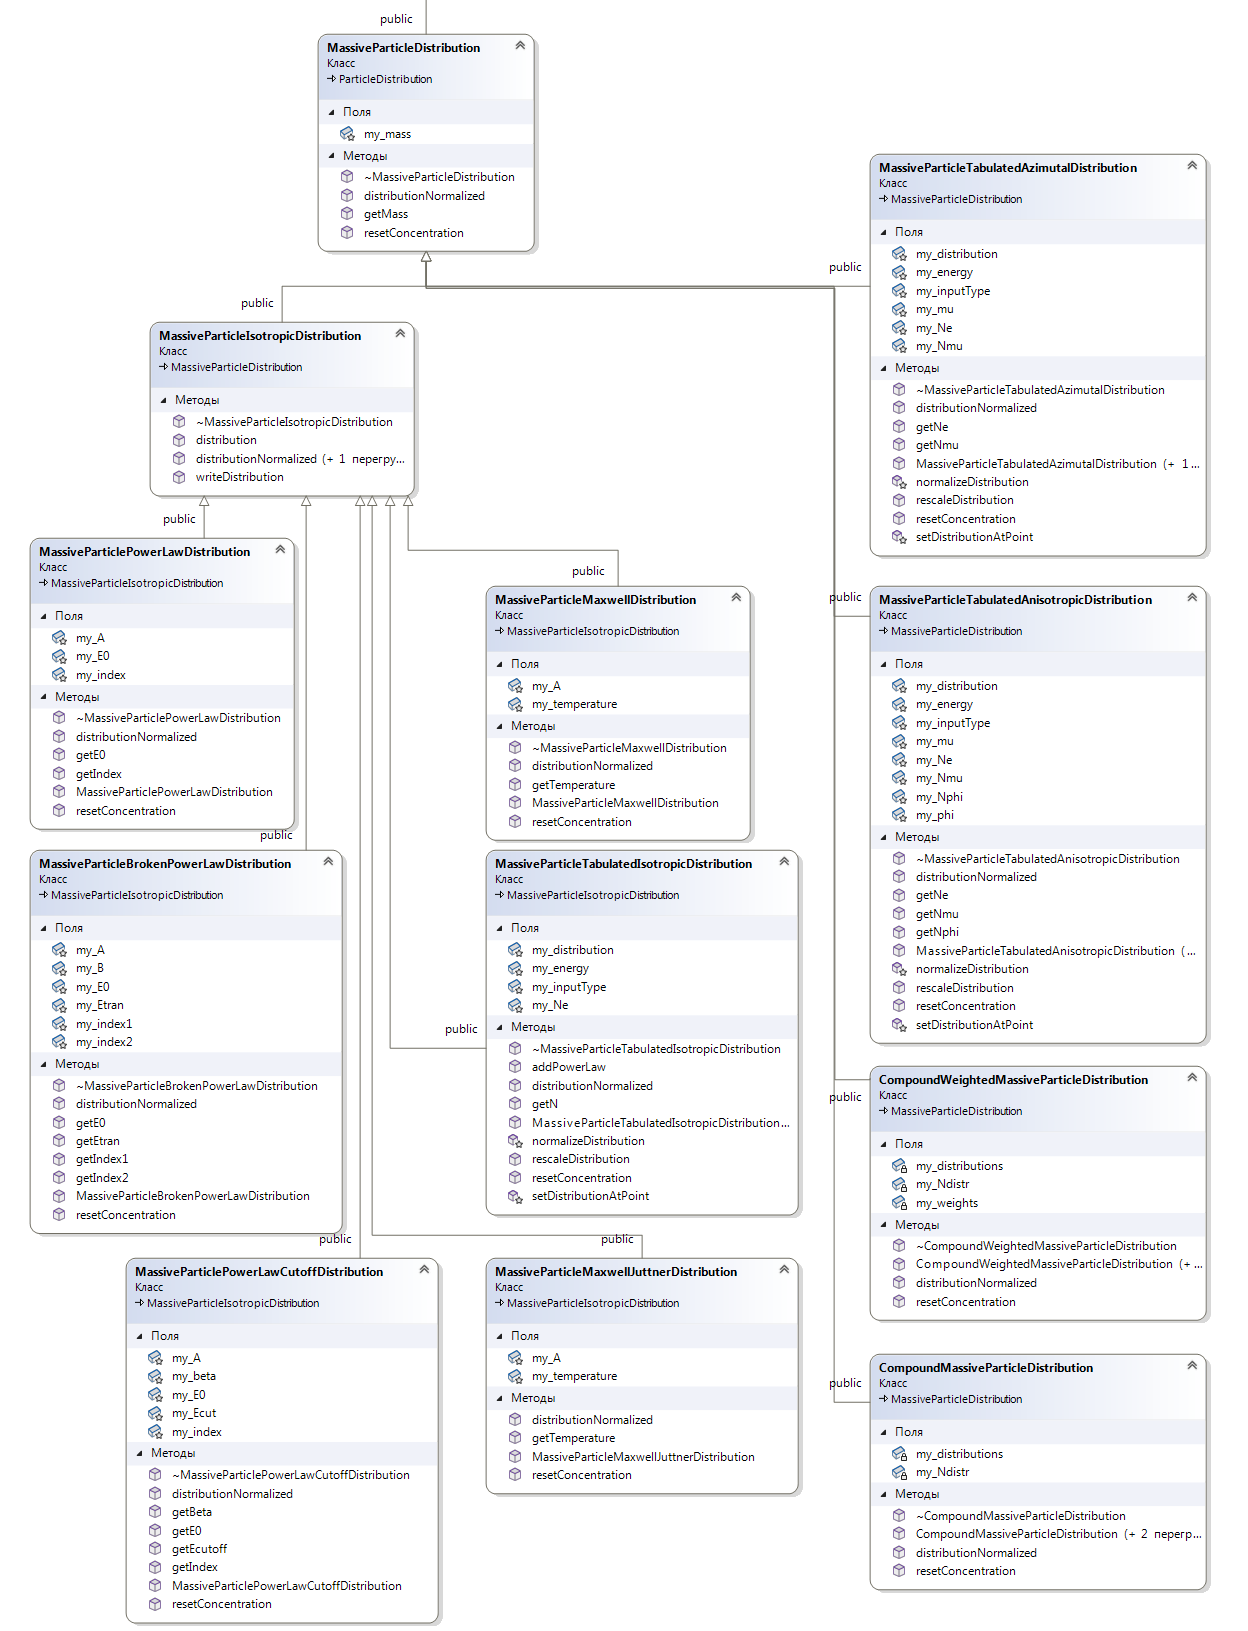
\includegraphics[width=14.5 cm]{./fig/massiveParticleDistribution1.png} 
	\caption{Схема наследования классов распределения массивных частиц}
	\label{massiveDistribution}
\end{figure}

Абстрактный класс изотропных распределений имеет шесть наследников, предназначенных для создания конкретных распределений: MassiveParticlePowerLawDistribution - для степенных распределений, MassiveParticleBrokenPowerLawDistribution - для степенных распределений с изломом, MassiveParticlePowerLawCutoffDistribution - для степенных распределений с экспоненциальным завалом, MassiveParticleMaxwellDistribution - для максвелловского распределения (обратите внимание, что в отличие от остальных распределений, максвелловское подразумевает под энергией только кинетическую энергию), MassiveParticleMaxwellJuttnerDistribution - для релятивистского распределения Максвелла-Юттнера и MassiveParticleTabulatedIsotropicDistribution - для таблично заданных распределений. 

Так же имеется четыре реализации анизотропных распределений: MassiveParticleTabulatedPolarDistribution - для таблично заданных распределений с зависимостью только от энергии и полярного угла, MassiveParticleAnisotropicDistribution - для таблично заданных распределений с зависимостью от всех переменных, CompoundMassiveParticleDistribution - для суммы распредлений общего вида, CompoundWeightedMassiveParticleDistribution - для взвешенной суммы распределений общего вида. В некоторых случаях оперировать весами распределений удобнее, чем непосредственно концентрациями. Полная схема наследования классов распределений массивных частиц представлена на рисунке \ref{massiveDistribution}, список публичных методов классов распределений массивных частиц приведен в Таблице \ref{MassiveParticleMethods1}. Пользователь может сам реализовывать необходимые ему виды распределений излучающих частиц, создав наследника класса MassiveParticleDistribution или MassiveParticleIsotropicDistribution и определив необходимые виртуальные методы.

\subsection{Считывание распределений из файла}
Классы таблично-заданных распределений, такие как например MassiveParticleTabulatedIsotropicDistribution, имеют конструктор принимающие на вход имена файлов, из которых будет считана функция распределения. Это должны быть текстовые файлы, содержащие таблицы с данными, причем формат единиц, в которых измеряется функция распределения может быть разным. Для задания формата входных файлов используется перечислимы тип DistributionInputType, имеющий пять значений:

\begin{itemize}
	\item ENERGY\_FE - во входных файлах заданы энергия и функция распределения по энергии
	\item ENERGY\_KIN\_FE - заданы кинетическая энергия и функция распределения по энергии
	\item GAMMA\_FGAMMA - задан лоренц-фактор и функция распределения по нему
	\item GAMMA\_KIN\_FGAMMA - задан лоренц-фактор, уменьшенный на единицу, и функция распределения по нему
	\item MOMENTUM\_FP - задан импульс и функция распределения по импульсу
\end{itemize}

Вне зависимости от формата входного файла, функция распределения будет преобразована к единицам энергия - распределение по энергии. С помощью этих параметров можно считывать табличные распределения из файлов, например так:

\begin{lstlisting}[language=c++]
	double electronConcentration = 1.0;
	int N = 100;
	MassiveParticleIsotropicDistribution* distribution = new
	MassiveParticleTabulatedIsotropicDistribution(massElectron,
	"energy.dat", "distribution.dat", N, electronConcentration,
	DistributionInputType::ENERGY_FE);
\end{lstlisting}

Для облегчения создания распределений из файла в сложных случаях реализован класс MassiveParticleDistributionFactory. У него есть несколько методов, позволяющих считывать целые серии распределений из набора пронумерованных файлов. Что может быть полезно, если функция распределения зависит от некоторого параметра, как в примере вычисления синхротронного излучения описанном в следующей главе \ref{}. Считать серию из десяти распределений электронов, содержащихся в файлах с именами  "Fe0.dat"\ , "Fe1.dat"\  и так далее, состоящих из двух колонок - лоренц-фактор и функция распределения, и добавить к этим распределениям степенной хвост с показателем 3, начиная с энергий в 100 энергий покоя можно вызовом одной функции: 

\begin{lstlisting}[language=c++]
	double electronConcentration = 1.0;
	int Nenergy = 100;
	int Ndistribution = 100;
	double powerLawEnergy = 100*me_c2;
	double index = 3.0;
	MassiveParticleIsotropicDistribution** distributions = 
	MassiveParticleDistributionFactory::
	readTabulatedIsotropicDistributionsAddPowerLawTail(
	massElectron, "./input/Fe", ".dat", Ndistribution, 
	DistributionInputType::GAMMA_FGAMMA, electronConcentration, Nenergy,
	powerLawEnergy, index);
\end{lstlisting}

Так же у пользователя есть возможность использовать конструкторы табличных распределений, принимающие не имена файлов, а непосредственно массивы со значениями функции распределения, которые пользователь создать любым удобным ему способом.

\begin{small}
	\topcaption{Публичные методы классов распределений массивных частиц }
	\label{MassiveParticleMethods1}
	\begin{xtabular}{|p{0.52\textwidth}|p{0.48\textwidth}|}
		\hline
		\textbf{MassiveParticlePowerLawDistribution} & Класс для степенного распределения\\
		\hline
		MassiveParticlePowerLawDistribution( const double\& mass, const double\& index, const double\& E0, const double\& concentration) & конструктор, создает экземпляр степенного распределния частиц с заданными массой, степенным индексом, начальной энергией распределения и полной концентрацией\\
		\hline
		getIndex() & возвращает степенной индекс распределения\\
		\hline
		getE0() & возвращает начальную энергию распределения\\
		\hline
		\textbf{MassiveParticleBrokenPowerLawDistribution} & Класс для степенного распределения с изломом\\
		\hline
		MassiveParticleBrokenPowerLawDistribution( const double\& mass, const double\& index1, const double\& index2, const double\& E0, const double\& Etran, const double\& concentration) & конструктор, создает экземпляр степенного распределния с изломом частиц с заданными массой, степенными индексоми на низких и высоких энергиях, начальной энергией распределения, энергией соответствующей излому и полной концентрацией\\
		\hline
		getIndex1() & возвращает степенной индекс распределения на низких энергиях\\
		\hline
		getIndex2() & возвращает степенной индекс распределения на высоких энергиях\\
		\hline
		getE0() & возвращает начальную энергию распределения\\
		\hline
		getEtran() & возвращает энергию излома\\
		\hline
		\textbf{MassiveParticlePowerLawCutoffDistribution} & Класс для степенного распределения с экспоненциальным завалом\\
		\hline
		MassiveParticlePowerLawCutoffDistribution(const double\& mass, const double\& index, const double\& E0, const double\& beta, const double\& Ecut, const double\& concentration) & конструктор, создает экземпляр степенного распределния с экспоненциальным завалом частиц с заданными массой, степенным индексом, начальной энергией распределения, параметром завала, энергией завала и полной концентрацией. $F(E)\propto (E/E_0)^{-index}\cdot\exp(-(E/E_{cut})^\beta)$\\
		\hline
		getIndex() & возвращает степенной индекс распределения \\
		\hline
		getBeta() & возвращает параметр завала распределения \\
		\hline
		getE0() & возвращает начальную энергию распределения\\
		\hline
		getEcutoff() & возвращает энергию экспоненциального завала\\
		\hline
		\textbf{MassiveParticleMaxwellDistribution} & Класс для распределения Максвелла\\
		\hline
		MassiveParticleMaxwellDistribution( const double\& mass, const double\& temperature, const double\& concentration) & конструктор, создает экземпляр распределния Максвелла частиц с заданными массой, температурой и полной концентрацией\\
		\hline
		getTemperature() & возвращает температуру распределения\\
		\hline
		\textbf{MassiveParticleMaxwellJuttnerDistribution} & Класс для распределения Максвелла-Юттнера\\
		\hline
		MassiveParticleMaxwellJuttnerDistribution( const double\& mass, const double\& temperature, const double\& concentration) & конструктор, создает экземпляр распределния Максвелла-Юттнера частиц с заданными массой, температурой и полной концентрацией\\
		\hline
		getTemperature() & возвращает температуру распределения\\
		\hline
		\textbf{MassiveParticleTabulatedIsotropicDistribution} & Класс для таблично заданного изотропного распределения\\
		\hline
		MassiveParticleTabulatedIsotropicDistribution( const double\& mass, const char* fileName, const int N, const double\& concentration, DistributionInputType inputType) & конструктор, создает экземпляр табличного распределния частиц с заданными массой и полной концентрацией с помощью указанного файла, состоящего из двух колнок с данными указанной длины. Так же указывается формат входных данных.\\
		\hline
		MassiveParticleTabulatedIsotropicDistribution( const double\& mass, const char* energyFileName, const char* distributionFileName, const int N, const double\& concentration, DistributionInputType inputType) & конструктор, создает экземпляр табличного распределния частиц с заданными массой и полной концентрацией с помощью указанных двух файлов, состоящих из колнок с данными указанной длины. Так же указывается формат входных данных. \\
		\hline
		MassiveParticleTabulatedIsotropicDistribution( const double\& mass, const double* energy, const double* distribution, const int N, const double\& concentration, DistributionInputType inputType) & конструктор, создает экземпляр табличного распределния частиц с заданными массой и полной концентрацией с помощью двух переданных массивов данных указанной длины. Так же указывается формат входных данных.\\
		\hline
		getN() & возвращает количество ячеек в таблице задающей функцию\\
		\hline
		getEmin() & возвращает минимальную энергию распределения\\
		\hline
		getEmax() & возвращает максимальную энергию распределения\\
		\hline
		rescaleDistribution(const double\& k) & масштабирует распределение, вытягивая его по оси энергии по формуле $E' = mc^2 + k\cdot(E-mc^2)$, $F(E')=F(E)/k$. Данная функция может быть полезна, например, в случае когда исходная функция распределения получена в результате работы численного кода с измененной массой электронов\\
		\hline
		addPowerLaw( const double\& Epower, const double\& index) & добавляет к функции распределения степенной с указанным индексом, начиная с указанной энергии. Функция распределения при этом остается нормированной на указанную ранее концентрацию\\
		\hline 
		\textbf{MassiveParticleTabulatedPolarDistribution} & Класс для таблично заданного распределения с зависимостью от полярного угла\\
		\hline
		MassiveParticleTabulatedPolarDistribution( const double\& mass, const char* energyFileName, const char* muFileName, const char* distributionFileName, const int Ne, const int Nmu, const double\& concentration, DistributionInputType inputType) & конструктор, создает экземпляр табличного распределния частиц с заданными массой и полной концентрацией с помощью  трех указанных файлов, в двух из которых содержатся сетки по энергии и косинусу полярного угла с указанными размерами, а в третьем двумерный массив функции распределения. Так же указывается формат входных данных.\\
		\hline
		MassiveParticleTabulatedPolarDistribution( const double\& mass, const double* energy, const double* mu, const double** distribution, const int Ne, const int Nmu, const double\& concentration, DistributionInputType inputType) & конструктор, создает экземпляр табличного распределния частиц с заданными массой и полной концентрацией с помощью трех переданных массивов данных, в двух из которых содержатся сетки по энергии и косинусу полярного угла с указанными размерами, а в третьем двумерный массив функции распределения. Так же указывается формат входных данных.\\
		\hline
		getNe() & возвращает количество ячеек по энергии в таблице задающей функцию распределения\\
		\hline
		getEmin() & возвращает минимальную энергию распределения\\
		\hline
		getEmax() & возвращает максимальную энергию распределения\\
		\hline
		getNmu() & возвращает количество ячеек по полярному углу в таблице задающей функцию распределения\\
		\hline
		rescaleDistribution(const double\& k) & масштабирует распределение, вытягивая его по оси энергии по формуле $E' = mc^2 + k\cdot(E-mc^2)$, $F(E',\mu)=F(E,\mu)/k$. Данная функция может быть полезна, например, в случае когда исходная функция распределения получена в результате работы численного кода с измененной массой электронов\\
		\hline
		\textbf{MassiveParticleTabulatedAnisotropicDistribution} & Класс для таблично заданного анизотропного распределения общего вида\\
		\hline
		MassiveParticleTabulatedAnisotropicDistribution( const double\& mass, const char* energyFileName, const char* muFileName, const char* distributionFileName, const int Ne, const int Nmu, const int Nphi, const double\& concentration, DistributionInputType inputType) & конструктор, создает экземпляр табличного распределния частиц с заданными массой и полной концентрацией с помощью  трех указанных файлов, в двух из которых содержатся сетки по энергии и косинусу полярного угла с указанными размерами, а в третьем двумерный массив функции распределения. Сетка по азимутальному углу считается расномерной и определяется только размером. Так же указывается формат входных данных.\\
		\hline
		MassiveParticleTabulatedAnisotropicDistribution( const double\& mass, const double* energy, const double* mu, const double*** distribution, const int Ne, const int Nmu, const int Nphi, const double\& concentration, DistributionInputType inputType) & конструктор, создает экземпляр табличного распределния частиц с заданными массой и полной концентрацией с помощью трех переданных массивов данных, в двух из которых содержатся сетки по энергии и косинусу полярного угла с указанными размерами, а в третьем двумерный массив функции распределения. Сетка по азимутальному углу считается расномерной и определяется только размером. Так же указывается формат входных данных.\\
		\hline
		getNe() & возвращает количество ячеек по энергии в таблице задающей функцию распределения\\
		\hline
		getEmin() & возвращает минимальную энергию распределения\\
		\hline
		getEmax() & возвращает максимальную энергию распределения\\
		\hline
		getNmu() & возвращает количество ячеек по полярному углу в таблице задающей функцию распределения\\
		\hline
		getNphi() & возвращает количество ячеек по азимутальному углу в таблице задающей функцию распределения\\
		\hline
		rescaleDistribution(const double\& k) & масштабирует распределение, вытягивая его по оси энергии по формуле $E' = mc^2 + k\cdot(E-mc^2)$, $F(E',\mu, \phi)=F(E,\mu, \phi)/k$. Данная функция может быть полезна, например, в случае когда исходная функция распределения получена в результате работы численного кода с измененной массой электронов\\
		\hline
		\textbf{CompoundMassiveParticleDistribution} & Класс для распределения, состоящего из суммы других распределений\\
		\hline
		CompoundMassiveParticleDistribution( int N, MassiveParticleDistribution** distributions) & конструктор, создает экземпляр класса содержащий смесь заданного количества указанных распределений\\
		\hline
		CompoundMassiveParticleDistribution( MassiveParticleDistribution* dist1, MassiveParticleDistribution* dist2) & конструктор, создает экземпляр класса, содержащий смесь двух распределений \\
		\hline
		CompoundMassiveParticleDistribution( MassiveParticleDistribution* dist1, MassiveParticleDistribution* dist2, MassiveParticleDistribution* dist3) & конструктор, создает экземпляр класса, содержащий смесь трех распределений\\
		\hline
		\textbf{CompoundWeightedMassiveParticleDistribution} & Класс для распределения, состоящего из взвешенной суммы других распределений \\
		\hline
		CompoundWeightedMassiveParticleDistribution( int N, const double* weights, MassiveParticleDistribution** distributions) & конструктор, создает экземпляр класса содержащий смесь заданного количества указанных распределений с заданными весами \\
		\hline
		CompoundWeightedMassiveParticleDistribution( MassiveParticleDistribution* dist1, const double\& w1, MassiveParticleDistribution* dist2, const double\& w2) & конструктор, создает экземпляр класса, содержащий смесь двух распределений с указанными весами \\
		\hline
		CompoundWeightedMassiveParticleDistribution( MassiveParticleDistribution* dist1, const double\& w1, MassiveParticleDistribution* dist2, const double\& w2, MassiveParticleDistribution* dist3, const double\& w3) & конструктор, создает экземпляр класса, содержащий смесь трех распределений с указанными весами \\
		\hline
				
	\end{xtabular}
\end{small}

\section{Источники излучения}

В коде FAINA есть возможность расчета излучения, используя на прямую функции распределения излучающих частиц, с указанием необходимых дополнительных параметров, таких как объем источника, расстояние до него, магнитное поле и других. Но более универсальным и рекомендованным способ является расчет с помощью создания модели источника излучения. При таком подходе возможно учесть геометрическое строение источника, его неоднородности и другие особенности.

Реализованы два базовых класса источников - независящие от времени, представленные абстрактным классом RadiationSource, и изменяющиеся со временем, представленные абстрактным классом RadiationTimeDependentSource. Эти два класса не связаны между собой через наследование, но объект первого класса содержится внутри объектов второго как приватное поле класса. Схема классов источников излучения представлена на рисунке \ref{radiationSource}.

\begin{figure}
	\centering
	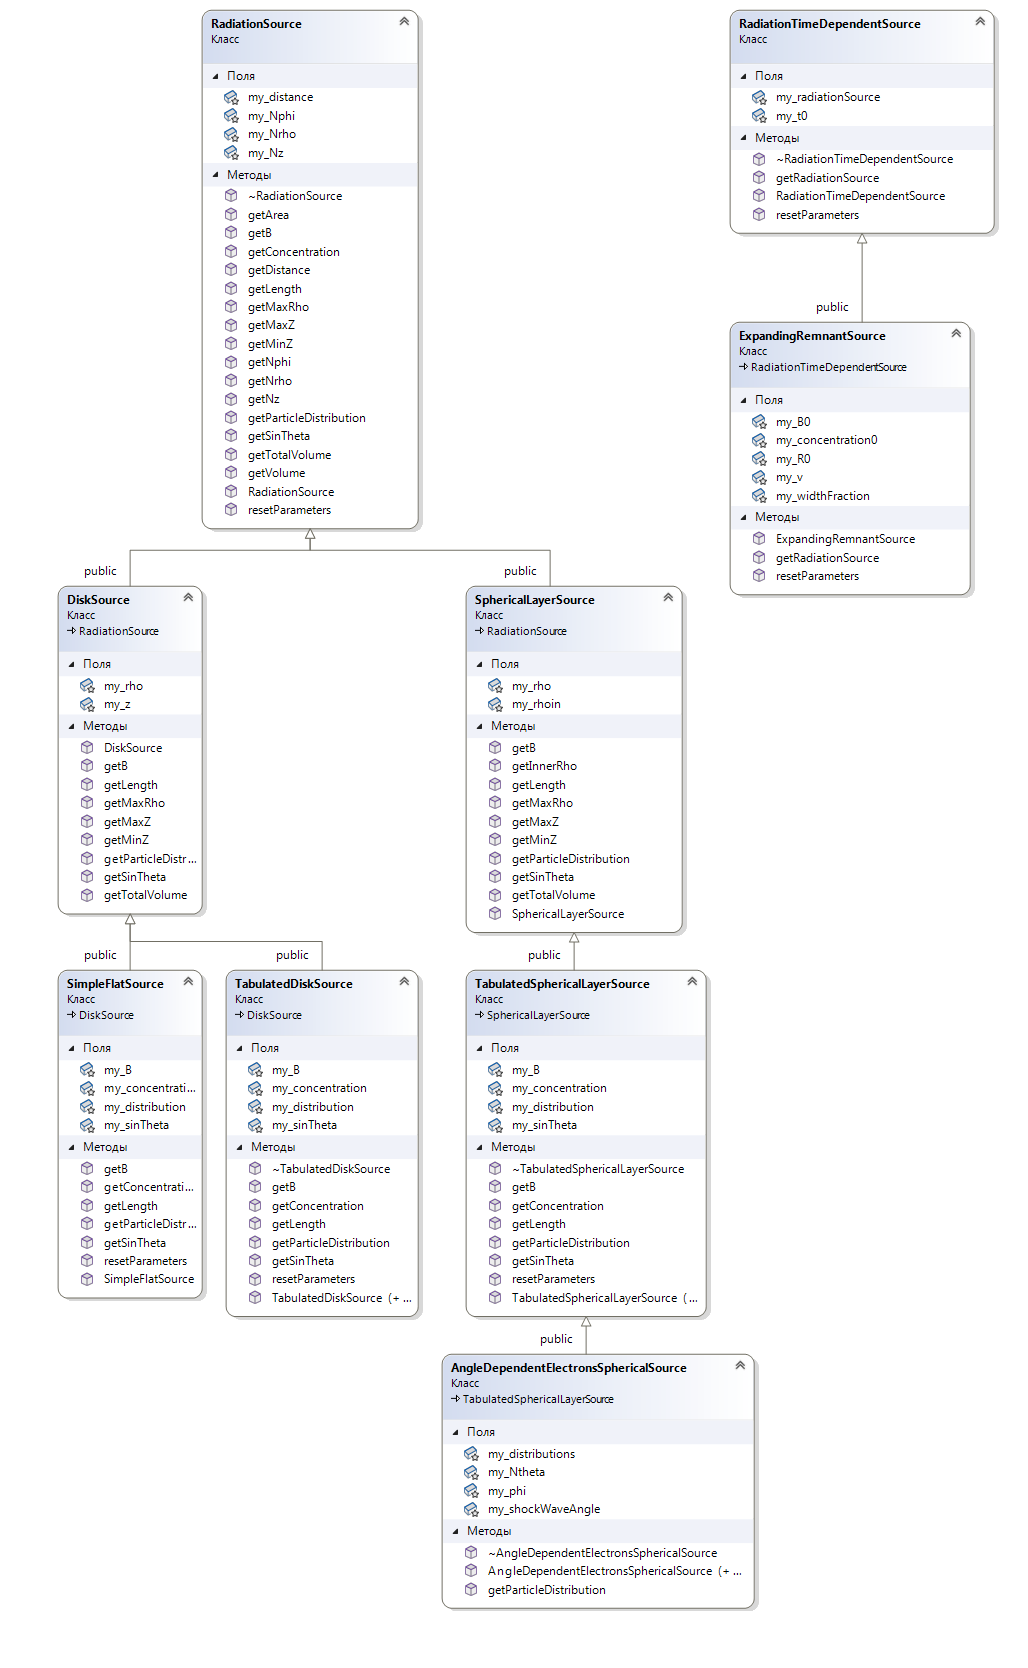
\includegraphics[width=14.5 cm]{./fig/radiationSource.png} 
	\caption{Схема наследования классов источников излучения}
	\label{radiationSource}
\end{figure}

\subsection{Источники излучения, не зависящие от времени}\label{sourcesSection}
Источники излучения без временной зависимости реализованы с помощью абстрактного класса RadiationSource. Геометрически каждый источник задан в виде пространственной области в цилиндрических координатах, с осью z направленной вдоль луча зрения к наблюдателю, и характеризуется максимальным радиусом и минимальным и максимальным значением координаты z. Такая система координат выбрана для удобства учета процессов поглощения при прохождении излучения внутри самого источника вдоль луча зрения. Отличие реальной формы источника от цилиндрической реализовано с помощью долей заполнения веществом источника ячеек пространственной сетки. Модель источника, имеющего форму шарового слоя, в цилиндрическо пространственной сетке изображена на рисунке \ref{sphericalLayer}. Цветом обозначена доля объема ячейки, заполненная веществом источника.

\begin{figure}
	\centering
	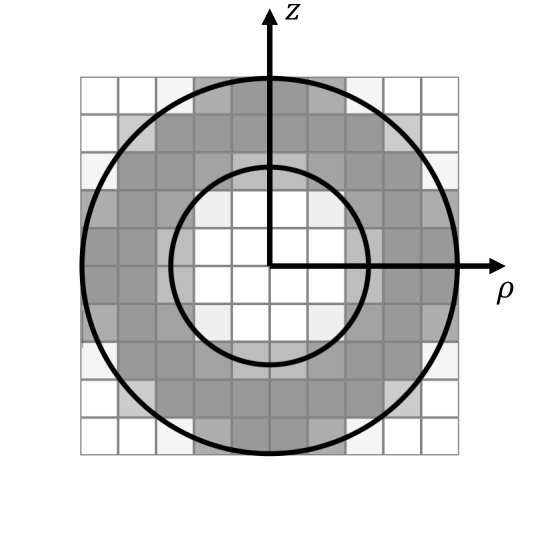
\includegraphics[width=10.5 cm]{./fig/sphericalSource.png} 
	\caption{Модель источника в форме шарового слоя, помещенного в цилиндрическую пространственную координатную сетку. Цвет характеризует долю объема ячейки, заполненную веществом источника.}
	\label{sphericalLayer}
\end{figure}

Так же источники излучения имеют следующие важные характеристки, которые могут меняться в различных пространственных ячейках источника: концентрация излучающих частиц, их функция распределения, магнитное поле и угол его наклона к лучу зрения. Большинство методов расчета излучения (все кроме обратного комптоновского рассеяния) реализованы только для изотропных распределений излучающих частиц, поэтому источники содержат только изотропные распределения. Так же у источника должно быть задано расстояние до наблюдателя.

Класс RadiationSource имеет два абстрактных класса-наследника: DiskSource - для источников в форме диска, перпендикулярного лучу зрения, и SphericalLayerSource - для источников в форме шарового слоя. Источники в форме диска имеют две реализации: SimpleFlatSource - однородный диск, состоящий из одной пространственной ячейки с заданными параметрами, и TabulatedDiskSource - источник, в котором все характеристики таблично заданы на пространственной сетке. Источники в форме шарового слоя имеют следующие реализации: TabulatedSphericalSource - источник, в котором все характеристики таблично заданы на пространственной сетке, и отнаследованный от него AngleDependentElectronsSphericalSource. Последний класс нужен для реализации важного в астрофизике случая, когда функция распределения излучающих частиц зависит от угла наклона магнитного поля по отношению к направлению распространения ударной волны \cite{SironiSpitkovsky2009pair, GuoSironi2014_1,Crumley2019, Romansky2018, еще}. В данном источнике такие параметры, как концентрация, магнитное поле и его угол наклона к лучу зрения заданы таблично на пространственной сетке, а функция распределения излучающих частиц - в виде таблицы по углам наклона магнитного поля к направлению распространения ударной волны, которая в данном случае считается сферически симметричной. Функция распределения в каждой ячейке выбирается в зависимости от вычисленного угла наклона магнитного поля к ударной волне. Публичные методы классов источников излучения без зависимости от времени перечислены в Таблице \ref{sourceMethods1}.

\begin{small}
	\topcaption{Публичные методы классов источников излучения без зависимости от времени }
	\label{sourceMethods1}
	\begin{xtabular}{|p{0.5\textwidth}|p{0.5\textwidth}|}
		\hline
		\textbf{RadiationSource} & абстрактный класс для источников излучения общего вида\\
		\hline
		virtual getMaxRho() & чисто виртуальный метод, возвращает максимальный цилиндрический радиус источника\\
		\hline
		virtual getMinZ() & чисто виртуальный метод, возвращает минимальную границу источника по оси z\\
		\hline
		virtual getMaxZ() & чисто виртуальный метод, возвращает максимальную границу источника по оси z\\
		\hline
		getNrho() & возвращает количество пространственных ячеек по радиальной оси цилиндрических координат\\
		\hline
		getNz() & возвращает количество пространственных ячеек по оси z цилиндрических координат\\
		\hline
		getNphi() & возвращает количество пространственных ячеек по по азимутальному углу цилиндрических координат\\
		\hline
		getDistance() & возвращает расстояние до источника\\
		\hline
		getArea(int irho) & возвращает поперечное сечение данной пространственной ячейки\\
		\hline
		getVolume(int irho, int iz, int iphi) & возвращает объем ячейки, занятый веществом источника. Этот метод согласован с методами getArea и getLength и возвращает их произведение\\
		\hline
		virtual getB(int irho, int iz, int iphi) & чисто виртуальный метод, возвращает значение магнитного поля в ячейке\\
		\hline
		virtual getConcentration(int irho, int iz, int iphi) & чисто виртуальный метод, возвращает значение концентрации в ячейке \\
		\hline
		virtual getSinTheta(int irho, int iz, int iphi) & чисто виртуальный метод, возвращает синус угла наклона магнитного поля к лучу зрения\\
		\hline
		virtual getTotalVolume() & чисто виртуальный метод, возвращает полный объем источника\\
		\hline
		virtual getLength(int irho, int iz, int iphi) & чисто виртуальный метод, возвращает среднюю толщину ячейки, заполненную веществом источника\\
		\hline
		virtual resetParameters(const double* parameters, const double* normalizationUnits) & чисто виртуальный метод, меняющий параметры источника. Список параметров, их количество, их влияние на источник определяются пользователем в конкретных реализациях класса. Принимет массив параметров и массив единиц в которых они измеряны. Данный метод используется в процедурах оптимизации, либо при учете изменения источника со временем\\
		\hline
		virtual getParticleDistribution(int irho, int iz, int iphi) & чисто виртуальный метод, возвращает распределение излучающих частиц в ячейке\\
		\hline
		\textbf{DiskSource} & Абстрактный класс для источников в форме диска\\
		\hline
		\textbf{SimpleFlatSource} & Класс для источников в форме однородного диска\\
		\hline
		SimpleFlatSource( MassiveParticleIsotropicDistribution* electronDistribution, const double\& B, const double\& sinTheta, const double\& rho, const double\& z, const double\& distance) & конструктор, возвращает экземпляр с заданными распределением частиц, магнитным полем, синусом угла его наклона, радиусом диска, толщиной диска и расстоянием до источника\\
		\hline
		\textbf{TabulatedDiskSource} & Класс для источников в форме диска с таблично заданными значениями параметров\\
		\hline
		TabulatedDiskSource( int Nrho, int Nz, int Nphi, MassiveParticleIsotropicDistribution* electronDistribution, double*** B, double*** sinTheta, double*** concentration, const double\& rho, const double\& z, const double\& distance) & конструктор, возвращает экземпляр с заданными с помощью массивов распределением частиц, магнитным полем, синусом угла его наклона, а так же заданными радиусом диска, толщиной диска и расстоянием до источника\\
		\hline
		TabulatedDiskSource( int Nrho, int Nz, int Nphi, MassiveParticleIsotropicDistribution* electronDistribution, const double\& B, const double\& sinTheta, const double\& concentration , const double\& rho, const double\& z, const double\& distance) & конструктор, возвращает экземпляр с заданными однородными распределением частиц, магнитным полем, синусом угла его наклона, а так же заданными радиусом диска, толщиной диска и расстоянием до источника\\
		\hline
		\textbf{SphericalLayerSource} & Абстрактный класс для источников в форме шарового слоя\\
		\hline
		double getInnerRho() & возвращает внутренний радиус шарового слоя\\
		\hline
		\textbf{TabulatedSphericalLayerSource} & Класс для источников в форме шарового слоя с таблично заданными значениями параметров\\
		\hline
		TabulatedSphericalLayerSource(int Nrho, int Nz, int Nphi, MassiveParticleIsotropicDistribution* electronDistribution, double*** B, double*** sinTheta, double*** concentration, const double\& rho, const double\& rhoin, const double\& distance) & конструктор, возвращает экземпляр с заданными с помощью массивов распределением частиц, магнитным полем, синусом угла его наклона к лучу зрения, а так же заданными внешним и внутренним радиусом диска и расстоянием до источника\\
		\hline
		TabulatedSphericalLayerSource(int Nrho, int Nz, int Nphi, MassiveParticleIsotropicDistribution* electronDistribution, const double\& B, const double\& concentration, const double\& sinTheta, const double\& rho, const double\& rhoin, const double\& distance) &  конструктор, возвращает экземпляр с заданными однородными распределением частиц, магнитным полем, синусом угла его наклона, а так же заданными внутренним и внешним радиусом диска и расстоянием до источника \\
		\hline
		\textbf{AngleDependentElectronsSphericalSource} & Класс для источников в форме шарового слоя с таблично заданными значениями концентрации и магнитного поля и функцией распределения излучающих частиц, зависящей от угла наклона магнитного поля к направлению распространения ударной волны\\
		\hline
		AngleDependentElectronsSphericalSource( int Nrho, int Nz, int Nphi, int Ntheta, MassiveParticleIsotropicDistribution** electronDistributions, double*** B, double*** sinTheta, double*** phi, double*** concentration, const double\& rho, const double\& rhoin, const double\& distance) & конструктор, возвращает экземпляр с заданными с помощью массивов магнитным полем, синусом угла его наклона к лучу зрения, а так же заданными внешним и внутренним радиусом диска и расстоянием до источника. Распределение частиц задается в виде массива табличных значений в зависимости от угла наклона магнитного поля к направлению распространения ударной волны\\
		\hline
		AngleDependentElectronsSphericalSource(int Nrho, int Nz, int Nphi, int Ntheta, MassiveParticleIsotropicDistribution** electronDistributions, const double\& B, const double\& sinTheta, const double\& phi, const double\& concentration, const double\& rho, const double\& rhoin, const double\& distance) & конструктор, возвращает экземпляр с заданными однородными  магнитным полем, синусом угла его наклона, а так же заданными внутренним и внешним радиусом диска и расстоянием до источника. Распределение частиц задается в виде массива табличных значений в зависимости от угла наклона магнитного поля к направлению распространения ударной волны\\
		\hline
	\end{xtabular}
\end{small}

\subsection{Источники излучения, меняющиеся со временем}\label{timeDependentSource}
Источники излучения, учитывающие зависимость от времени, представлены абастрактным классом классом RadiationTimeDependentSource. Этот класс не является наследником класса RadiationSource, но содержит экземпляр такого класса внутри себя, чтобы использовать его для расчета излучения в конкретный момент времени. Для этого пользователь должен самостоятельно создать имплементацию виртуальной функции getRadiationSource, в которой будут вычислены параметры источника в зависимости от времени.  В текущей версии кода реализован только один наследник RadiationTimeDependentSource - ExpandingRemnantSource, представляющий собой модель расширяющегося остатка сверхновой. В данной модели предполагается, что размер источника увеличивается во времени с постоянной скоростью, магнитное поле падает обратно пропорционально размеру источника, концентрация обратно пропорционально квадрату размера а толщина шарового слоя остается постоянной. Пользователь может создавать свои классы источников с другими зависимостями параметров от времени. Публичные методы классов RadiationTimeDependentSource и ExpandingRemnantSource перечислены  в Таблице \ref{sourceTimeDependentMethods1}.

\begin{small}
	\topcaption{Публичные методы классов источников излучения учитывающих зависимость от времени }
	\label{sourceTimeDependentMethods1}
	\begin{xtabular}{|p{0.5\textwidth}|p{0.5\textwidth}|}
		\hline
		\textbf{RadiationTimeDependentSource} & Абстрактный класс для учета изменений источников излучения со временем\\
		\hline
		virtual resetParameters(const double* parameters, const double* normalizationUnits) & чисто виртуальный метод, меняющий параметры источника. Список параметров, их количество, их влияние на источник определяются пользователем в конкретных реализациях класса. Принимет массив параметров и массив единиц в которых они измеряны. Данный метод применяется в процедурах оптимизации\\
		\hline
		virtual getRadiationSource(double\& time, const double* normalizationUnits) & возвращает источник излучения с параметрами соответствующими заданному моменту времени. Так же принимает на вход массив единиц, в которых измеряются параметры этого источника.\\
		\hline
		\textbf{ExpandingRemnantSource} & класс, представляющий модель расширяющегося с постоянной скоростью остатка сверхновой, имеющего форму шарового слоя постоянной толщины с однородными концентрацией и магнитным полем \\
		\hline
		ExpandingRemnantSource(const double\& R0, const double\& B0, const double\& concentration0, const double\& v, const double\& widthFraction, RadiationSource* source, const double\& t0) & конструктор, создает экземпляр класса расширяющейся сферической оболочки с заданными в момент t0 радиусом, магнитным полем, концентрацией, скоростью расширения, отношением толщины оболочки к радиусу и моделью источника. Для коректного учета изменения источника во времени важно, чтобы конретная реализация метода source->resetParameters соответствовала той,что используется в методе getRadiationSource. В данном случае подходят все перечисленные выше реализации источников не зависящих от времени\\
		\hline
	\end{xtabular}
\end{small}

\section{Вычисление излучения}

Для расчета излучения источников используется класс RadiationEvaluator и его наследники. Список публичных методов этого класса приведен в Таблице \ref{radiationEvaluator}. Общая схема расчета излучения такова: создать источник излучения, используя один из классов описанных в предыдущем разделе или написанный самостоятельно, затем создать вычислитель излучения нужного типа, и вызвать у него метод evaluateFluxFromSource(const double\& photonFinalEnergy, RadiationSource* source), вычисляющую энергетическую плотность потока излучения источника на данной энергии принимаемого фотона в единицах  $\text{см}^{-2} \text{с}^{-1}$. Далее в данном разделе описаны реализации класса RadiationEvaluator для конкретных видов излучения. Схема наследования классов вычислителей излучения представлена на рисунке \ref{radiationEvaluators}. Физическая сторона вопроса, формулы по которым расчитывается излучение подробно описаны в Главе \ref{Formulae}.

\begin{table}
	\begin{center}
		\begin{small}
	\caption{Публичные методы классa RadiationEvaluator }
	\label{radiationEvaluator}
	\begin{xtabular}{|p{0.5\textwidth}|p{0.5\textwidth}|} 
		\hline
		\textbf{RadiationEvaluator} & абстрактный класс для вычисления излучения \\
		\hline
		virtual evaluateFluxFromIsotropicFunction( const double\& photonFinalEnergy, MassiveParticleIsotropicDistribution* electronDistribution, const double\& volume, const double\& distance) & чисто виртуальный метод, возвращает энергетическую плотность потока излучаемого элементарным объемом с источника с данным распределением, на данном расстоянии от наблюдателя в единицах $\text{см}^{-2} \text{с}^{-1}$. Данный метод лучше не использовать самостоятельно, использовать вместо него расчет излучения от источников\\
		\hline
		virtual evaluateFluxFromSource(const double\& photonFinalEnergy, RadiationSource* source) & чисто виртуальный метод, возвращает энергетическую плотность потока излучаемого данным источником в единицах $\text{см}^{-2} \text{с}^{-1}$ \\
		\hline
		virtual resetParameters( const double* parameters, const double* normalizationUnits) & чисто виртуальный метод, позволяет изменить внутренние параметры вычислителя излучения. Список параметров, их количество, их влияние на источник определяются  в конкретных реализациях класса, данный метод используется при оптимизации\\
		\hline
		writeFluxFromSourceToFile(const char* fileName, RadiationSource* source, const double\& Ephmin, const double\& Ephmax, const int Nph) & записывает в файл с данным именем излучение источника в единицах $\text{см}^{-2} \text{с}^{-1}$ в диапазоне от минимальной до максимальной энергии, с заданным количеством точек, распределенных логарифмически\\
		\hline
	\end{xtabular}
\end{small}
\end{center}
\end{table}

\begin{figure}
	\centering
	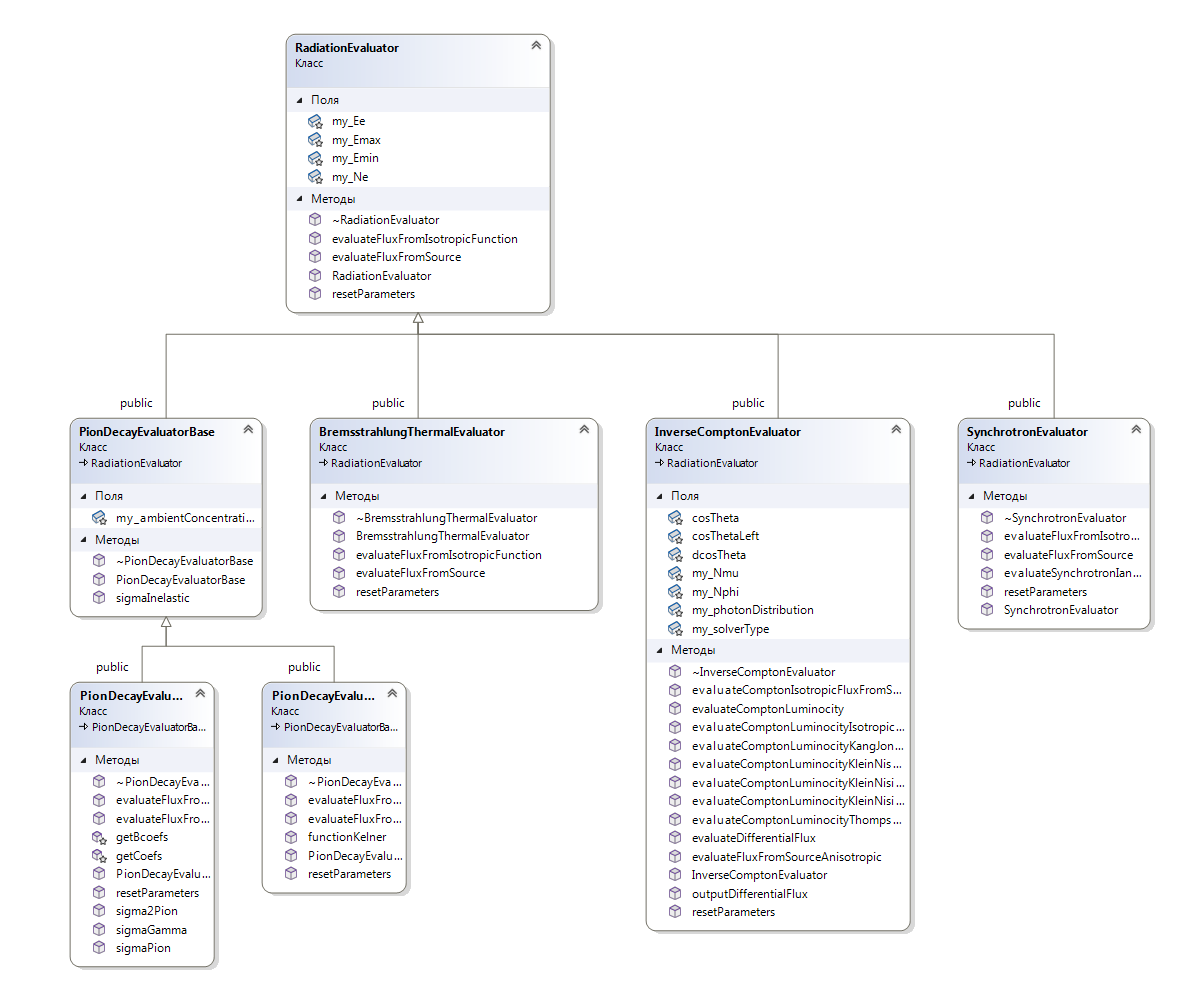
\includegraphics[width=10.5 cm]{./fig/radiationEvaluator.png} 
	\caption{Схема наследования классов вычислителей излучения.}
	\label{radiationEvaluators}
\end{figure}

\subsection{Синхротронное излучение}
Для расчета синхротронного излучения используется класс SynchrotronEvaluator. В нем используется приближение непрерывного спектра, то есть рассматриваемые частоты фотонов предполагаются намного большими, чем частота вращения излучающих частиц в магнитном поле. Реализован случай только изотропной функции распределения излучающих частиц. Так же возможен учет синхротронного самопоглощения. Используемая геометрия источников, показанная на рисунке \ref{sphericalLayer}, позволяет легко интегрировать излучение по лучу зрения, и учитывать при этом поглощение внутри источника. При создании объекта класса необходимо указать рассматриваемый диапазон энергий частиц и количество точек в нем, параметр отвечающиза учет самопоглощения (значение по умолчанию true), а так же значения магнитного поля, синуса угла наклона к лучу зрения и толщины излучаемой области, которые будут использоваться в случае расчета излучения без указания источника, а только с использованием распределения частиц. Публичные методы класса SynchrotronEvaluator перечислены в Таблице \ref{SynchrotronEvaluator}. Пример вычисления синхотронного излучения приведен в разделе \ref{quickStart}.
\begin{table}
	\begin{center}
	\begin{small}
	\caption{Публичные методы классa SynchrotronEvaluator }
	\label{SynchrotronEvaluator}
	\begin{tabularx}{\textwidth}{|X|X|} 
		\hline
		\textbf{SynchrotronEvaluator} & класс предназначенный для вычисления синхротронного излучения\\
		\hline
		SynchrotronEvaluator( int Ne, double Emin, double Emax, bool selfAbsorption = true, const double\& defaultB = 0, const double\& defaultSinTheta = 1.0, const double\& defaultLength = 0) & конструктор, создает экземпляр с указанным диапазоном рассматриваемых энергий, параметром учета самопоглощения, и значениями по умолчанию магнитного поля, его наклона и толщины\\
		\hline
		evaluateSynchrotronIandA(const double\& photonFinalFrequency, const double\& photonFinalTheta, const double\& photonFinalPhi, const double\& B, const double\& sinhi, const double\& concentration, MassiveParticleIsotropicDistribution* electronDistribution, double\& I, double\& A) & вычисляет значения излучательной способности и коэффициента поглощения распределения с данной концентрацией в данном магнитном поле\\
		\hline
	\end{tabularx}
\end{small}
\end{center}
\end{table}
\subsection{Обратное комптоновское рассеяние}
Для расчета излучения, получающегося в результате процесса обратного комптоновского рассеяния, использеутся класс InverseComptonEvaluator. Внутри него реализованы четыре различных метода расчета излучения, для обозначения которых используется перечислимый тип ComptonSolverType, имеющий следующие значения:

\begin{itemize}
	\item ISOTROPIC\_THOMSON - модель рассеяния в томсоновсков режиме. Реализовано только для степенного распределения электронов и теплового фотонов \cite{Ginzburg1975} глава 17, с 466
	\item ANISOTROPIC\_KLEIN\_NISHINA - модель расчитывающее излучение напрямую из сечения Клейна-Нишины, возможен учет анизотропных функций распределения \cite{KleinNishina, Dubus}
	\item ISOTROPIC\_KLEIN\_NISHINA - модель расчитывающее излучение напрямую из сечения Клейна-Нишины, но для изотропных функций распределения, что позволяет уменьшить количество интегрирований
	\item ISOTROPIC\_JONES - модель, использующая аналитически проинтегрированное по углам сечение Клейна-Нишины \cite{JonesCompton, BykovUvarov2000}
\end{itemize}

При создании объекта класса InverseComptomEvaluator необходимо указать рассматриваемый диапазон энергий частиц и количество точек в нем, количество ячеек в сетке по полярному и азимутальному углу, изотропную функцию распределения фотонов, которая будет использоваться по умолчанию и метод расчета излучения. Публичные методы класса SynchrotronEvaluator перечислены в Таблице \ref{InverseComptonEvaluator}.
\begin{table}[h]
	\begin{center}
		\begin{small}
	\caption{Публичные методы классa InverseComptonEvaluator }
	\label{InverseComptonEvaluator}
	\begin{tabularx}{\textwidth}{|X|X|} 
		\hline
		\textbf{InverseComptonEvaluator} & класс предназначенный для вычисления излучения рождащегося в результате обратного комптоновского рассеяния\\
		\hline
		InverseComptonEvaluator( int Ne, int Nmu, int Nphi, double Emin, double Emax, PhotonIsotropicDistribution* photonDistribution, ComptonSolverType solverType) & конструктор, создает экземпляр с заданным рассматриваемым диапазоном энергии, количеством ячеек в сетке по полярному и азимутальному углу, изотропной функцией распределения фотонов, которая будет использоваться по умолчанию и методом расчета излучения\\
		\hline
		evaluateComptonFluxKleinNishinaAnisotropic const double\& photonFinalEnergy, const double\& photonFinalTheta, const double\& photonFinalPhi, PhotonDistribution* photonDistribution, MassiveParticleDistribution* electronDistribution, const double\& volume, const double\& distance) & возвращает энергетическую плотность потока энергии в заданном направлении, излучением созданным заданными функциями распределения фотонов и рассеивющих частиц (которые могут быть анизотропными) в заданном объеме на данном расстоянии\\
		\hline
		evaluateFluxFromSourceAnisotropic( const double\& photonFinalEnergy, const double\& photonFinalTheta, const double\& photonFinalPhi, PhotonDistribution* photonDistribution, RadiationSource* source) & возвращает энергетическую плотность потока энергии в заданном направлении, излучением созданным заданными распределения фотонов и источником, содержащим распределения рассеивающих частиц\\
		\hline
	\end{tabularx}
\end{small}
\end{center}
\end{table}

Пример вычисления излучения от обратного комптоновского рассеяние содержится в процедуре evaluateComtonWithPowerLawDistribution() в файле main.cpp. В ней расчитывается рентгеновское излучение, исходящее от объекта CSS161010 при рассеивании степенного распределения электронов, определенного в работе \cite{Coppejans2020}, на среднегалактическом распределении фотонов.  Сначала определим переменные, задающие основные параметры источника - концентрацию частиц, его размер и магнитное поле. Для вычисления обратного комптоновского рассеяния магнитное поле не используется, но в источнике нужно его задать, поэтому положим его равным нулю. Так же зададим параметры сетки по энергиям и углам, которая будет использоваться вычислителем

\begin{lstlisting}[language=c++]
	double electronConcentration = 150;
	double sinTheta = 1.0;
	double rmax = 1.3E17;
	double B = 0.0;
	double distance = 150*1E6*parsec;
	
	double Emin = me_c2;
	double Emax = 1000 * me_c2;
	int Ne = 200;
	int Nmu = 20;
	int Nphi = 4;
\end{lstlisting}

Далее создадим распределение фотонов, воспользовавшись статическим методом класса MultiPlankDistribution getGalacticField, который возвращает среднегалактическое фотонное распределение, и распределение электронов - возьмем степенное рспределение с показателем 3.5.
\begin{lstlisting}[language=c++]
	PhotonIsotropicDistribution* photonDistribution = 
	    PhotonMultiPlankDistribution::getGalacticField();
	MassiveParticlePowerLawDistribution* electrons = new 
	    MassiveParticlePowerLawDistribution(massElectron, 3.5,
	    Emin, electronConcentration);
\end{lstlisting}

С помощью введенных ранее переменных создадим источник излучения и вычислитель излучения. В качестве метода расчета выберем самый универсальный - ANISOTROPIC\_KLEIN\_NISHINA

\begin{lstlisting}[language=c++]
	RadiationSource* source = new SimpleFlatSource(
	  electrons, B, sinTheta, rmax, rmax, distance);
	
	InverseComptonEvaluator* comptonEvaluator = new 
	    InverseComptonEvaluator(Ne, Nmu, Nphi, Emin, Emax, 
	    photonDistribution, ComptonSolverType::ANISOTROPIC_KLEIN_NISHINA);
\end{lstlisting}

Предположим, что мы не хотим пользоваться встроенным методом вывода излучения в файл, так как хотим получить конечный результат в других единицах, например энергию фотона измерят в электронвольтах, а поток вывести в формате $E F(E)$ - $\text{эрг}\text{см}^{-2}\text{с}^{-1}$. Создадим тогда сетку значений энергии фотонов
\begin{lstlisting}[language=c++]
	int Nnu = 200;
	double* E = new double[Nnu];
	double* F = new double[Nnu];
	double Ephmin = 0.01 * kBoltzman * 2.725;
	double Ephmax = 2 * Emax;
	double factor = pow(Ephmax / Ephmin, 1.0 / (Nnu - 1));
	E[0] = Ephmin;
	F[0] = 0;
	for (int i = 1; i < Nnu; ++i) {
		E[i] = E[i - 1] * factor;
		F[i] = 0;
	}
\end{lstlisting}
после этого вычислим в цикле желаемые потоки излучения
\begin{lstlisting}[language=c++]
	for (int i = 0; i < Nnu; ++i) {
		F[i] = comptonEvaluator->evaluateFluxFromSource(
		    E[i], source);
	}
\end{lstlisting}
и запишем их в файл, переведя в желаемые единицы
\begin{lstlisting}[language=c++]
	FILE* output_ev_EFE = fopen("output.dat", "w");
	
	for (int i = 0; i < Nnu; ++i) {
		double nu = E[i] / hplank;
		fprintf(output_ev_EFE, "%g %g\n",
		    E[i] / (1.6E-12), E[i] * F[i]);
	}

	fclose(output_ev_EFE);
\end{lstlisting}
Спектр излучения, полученный в результате работы данной программы приведен на рисунке \ref{compton}
\begin{figure}
	\centering
	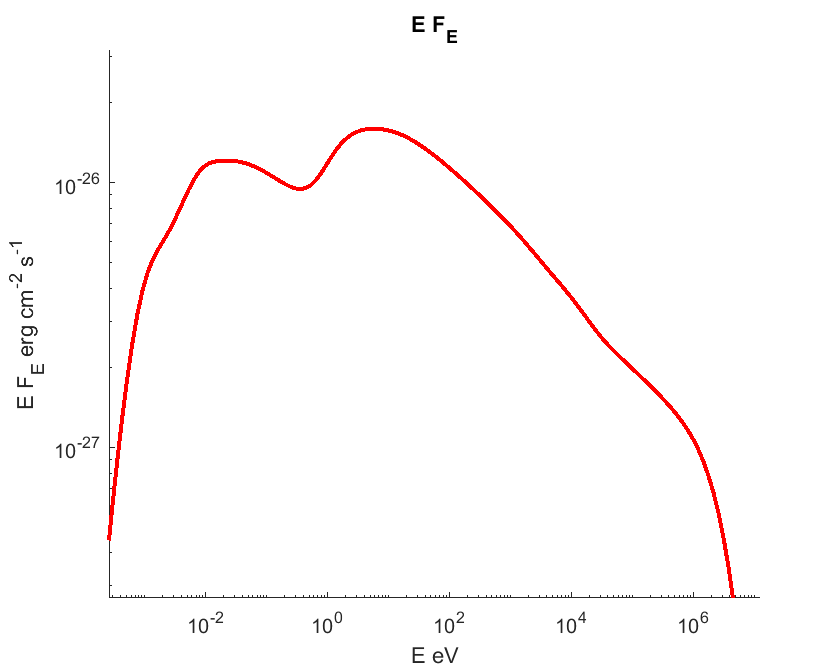
\includegraphics[width=12.5 cm]{./fig/compton.png} 
	\caption{Энергетическая плотность потока синхротронного излучения от тестового источника}
	\label{compton}
\end{figure}

\subsection{Распад пионов}

Для расчета излучения, получающегося в результате распада пионов, родившихся в результате свободно-свободного взаимодействия протонов использеутся абастрактный класс PionDecayEvaluatorBase и двае его наследника: PionDecayEvaluatorKelner, в котором сечение излучения гамма-фотона считается долей от полного сечения неупругого взаимодействия протонов, как описано в статье \cite{Kelner}, и PionDecayEvaluator, в котором используется более точное описание сечения рождения пионов на низких энергиях по методу, описанному в \cite{Kafexhiu}. При создании объекта класса InverseComptomEvaluator необходимо указать рассматриваемый диапазон энергий частиц и количество точек в нем, а так же концентрацию фоновых протонов, так как предполагается рассеяние высокоэнергичных фотонов на покоящихся, а не взаимодействие высокоэнергичных между собой. Публичные методы класса PionDecayEvaluatorBase и его наследников приведены в Таблице \ref{pionDecay}

\begin{table}[h]
	\begin{center}
		\begin{small}
			\caption{Публичные методы классa PionDecayEvaluatorBase и его наследников }
			\label{pionDecay}
			\begin{tabularx}{\textwidth}{|X|X|} 
				\hline
				\textbf{PionDecayEvaluatorBase} & абстрактный класс для вычисления гамма излучения от распада пионов\\
				\hline
				sigmaInelastic(const double\& energy) & возвращает полное сечение неупругого взаимодействия протонов в лабораторной системе, принимает кинетическую энергию движущегося протона\\
				\hline
				\textbf{PionDecayEvaluatorKelner} & класс для вычисления гамма излучения от распада пионов по методу из статьи \cite{Kelner}\\
				\hline
				PionDecayEvaluatorKelner(int Ne, double Emin, double Emax, const double\& ambientConcentration) & конструктор, создает экземпляр с заданным рассматриваемым диапазоном энергии и концентрацией фоновых протонов\\
				\hline
				\textbf{PionDecayEvaluator} & класс для вычисления гамма излучения от распада пионов по методу из статьи \cite{Kafexhiu}\\
				\hline
				PionDecayEvaluator(int Ne, double Emin, double Emax, const double\& ambientConcentration) & конструктор, создает экземпляр с заданным рассматриваемым диапазоном энергии и концентрацией фоновых протонов\\
				\hline
				sigmaGamma(const double\& photonEnergy, const double\& protonEnergy) & возвращает дифференциальное сечение рождения фотона с данной энергией при данной кинетической энергии протона, усредненное по углам\\
				\hline
			\end{tabularx}
		\end{small}
	\end{center}
\end{table}

Пример вычисления излучения от гамма излучения от распада пионов показан в функции evaluatePionDecay() в файлк main.cpp. В нем рассмотрено моделирование излучение объекта Кокон Лебедя в модели ускорения частиц на вторичных ударных волнах, следуя статье \cite{BykovKalyashova2022}. В данной работе вычислено, что спектр ускоренных протонов имеет вид степенной функции с изломом со следующими параметрами - показатели спектра 2.1 и 2.64 на низких и высоких энергиях соответственно, энергия излома - 2.2 ТэВ. Размер излучающей области брался равным размеру сверхкаверны Лебедя - 55 пк. Как и ранее, сначала определим переменные, задающие основные параметры источника - концентрацию частиц, его размер и магнитное поле, которое опять положим равным нулю. Диапазон энергий протонов рассмотрим от 0.01 ГэВ до 10 ТэВ. Так же укажем энергию излома.
\begin{lstlisting}[language=c++]
	double protonConcentration = 150;
	double rmax = 55 * parsec;
	double B = 0;
	double sinTheta = 1.0;

	double distance = 1400 * parsec;
	double Emin = massProton*speed_of_light2 + 0.01E9 * 1.6E-12;
	double Emax = 1E13 * 1.6E-12;
	double Etrans = 2.2E12 * 1.6E-12;
\end{lstlisting}
После этого создадим распределение протонов и источник излучения
\begin{lstlisting}[language=c++]
	MassiveParticleBrokenPowerLawDistribution* protons = new 
		MassiveParticleBrokenPowerLawDistribution(
		massProton, 2.1, 2.64, Emin, Etrans, protonConcentration);
	RadiationSource* source = new SimpleFlatSource(
		protons, B, sinTheta, rmax, rmax, distance);
\end{lstlisting}
Далее потребуется вычислитель излучения. В случае пионного распада необходимо указать концентрацию фоновых протонов.
\begin{lstlisting}[language=c++]
double protonAmbientConcentration = 20;
PionDecayEvaluator* pionDecayEvaluator = new PionDecayEvaluator(
	200, Emin, Emax, protonAmbientConcentration);
\end{lstlisting}
Как и в предыдущих случаях далее необходимо внутри цикла вычислить излучение в интересующем диапазоне энергий, используя функцию evaluateFluxFromSource, и вывести результат в файл в удобных единицах. Спектр излучения, полученный в результате работы данной программы и результаты наблюдений Кокона Лебедя на Fermi LAT, ARGO и HAWC \cite{Ackermann2011, Bartoli2014, Abeysekara2021} приведены на рисунке \ref{pion}
\begin{figure}
	\centering
	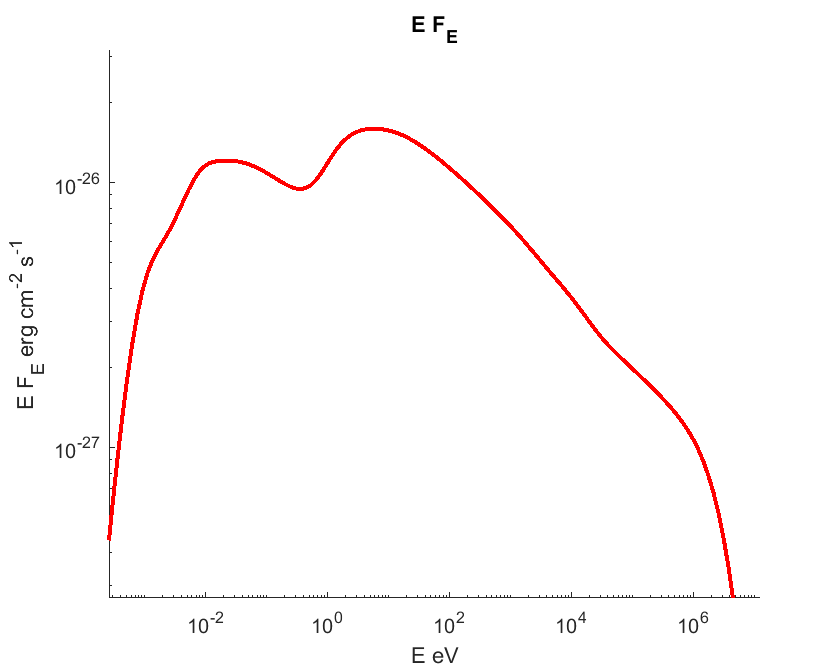
\includegraphics[width=12.5 cm]{./fig/compton.png} 
	\caption{Расчетная энергетическая плотность потока гамма излучения Кокона Лебедя и данные наблюдений}
	\label{pion}
\end{figure}
\subsection{Тормозное излучение}
В текущей версии кода реализовано вычисление тормозного излучения электронов в плазме только для случая теплового распределения. Для этого предназначен класс BremsstrahlungThermalEvaluator. В процессе расчета предполагается, что плазма электрон-протонная, с одинаковыми температурами электронов и протонов, в вычислении используются Гаунт-факторы, приведенные в \cite{Rybicki}. Пример вычисления тормохного излучения приведен в функции evaluateBremsstrahlung в файле main.cpp.

			% Глава 1. Расчет излучения источников
%\chapter{Оптимизация параметров}\label{optimization}
Код FAINA позволяет не только расчитывать излучение заданных источников, но и фитировать наблюдательные данные модельными, подбирая необходимые параметры. Реализованы методы оптимизации, пригодные для произвольного числа параметров и широкого класса моделей источников. В качестве целевой функции используется взвешенная сумма квадратов отклонений по всем наблюдательным точкам $f = \sum \frac{(F_i - F_{obs,i})^2}{\sigma_i^2}$, где $F_i$ - расчетная спектральная плотность потока излучения, $F_{obs,i}$ - наблюдаемая спектральная плотность потока излучения, $\sigma_i$ - её погрешность. В текущей версии учитывается лишь погрешность измеряемого потока, ширина бина и неопределенность энергии, на которой принят сигнал не учитываются.

Реализованные методы оптимизации делятся на два типа - те, которые рассматривают излучение в один момент времени, либо постоянные во времени, и те, которые учитывают эволюцию источников и используют наблюдения в разные моменты времени. В последнем случае пользователю необходимо самостоятельно указывать, как меняются параметры источника со временем, см. раздел \ref{timeDependentSource}.

\section{Фитирование источников, не зависящих от времени}
Для фитирования постоянных во времени кривых блеска предназначен абстрактный класс RadiationOptimizer. В нем определена виртуальныя функция optimize(double* vector, bool* optPar, double* energy, double* observedFlux, double* observedError, int Ne, RadiationSource* source), которая и производит процесс оптимизации. Входными параметрами являются: vector - массив подбираемых параметров, в который будет записан результат работы программы, optPar - массив булевских переменных, определяющих оптимизировать соответствующий параметр, или считать его фиксированным, energy - массив энергий, на которых производились наблюдения, observedFlux - соответствующие наблюдаемые потоки в единицах $\text{см}^{-2}\text{с}^{-1}$, Ne - количество наблюдательных точек, source - источник излучения. Функция изменения параметров источника source->resetParameters, описанная в разделе \ref{sourcesSection}, должна быть согласована с массивом оптимизируемых параметров vector, так как в процессе оптимизации он будет передаваться в нее в качестве аргумента.

В коде реализованы два наследника класса RadiationOptimazer: GridEnumRadiationOptimizer - производящий поиск минимума простым перебором по сетке параметров с заданным количеством распределенных равномерно логарифмически точек, и GradientDescentRadiationOptimizer - в котором минимум находится методом градиентного спуска. Эти два класса полезно использовать совместно, используя результат работы первого как начальную точку для второго. Схема насследования классов оптимизаторов показана на рисунке \ref{radiationOptimizer}, а список их публичных методов приведен в Таблице \ref{RadiationOptimizerMethods}. Реализованные методы оптимизации применимы для всех описанных выше типов источников и видов электромагнитного излучения.
\begin{figure}
	\centering
	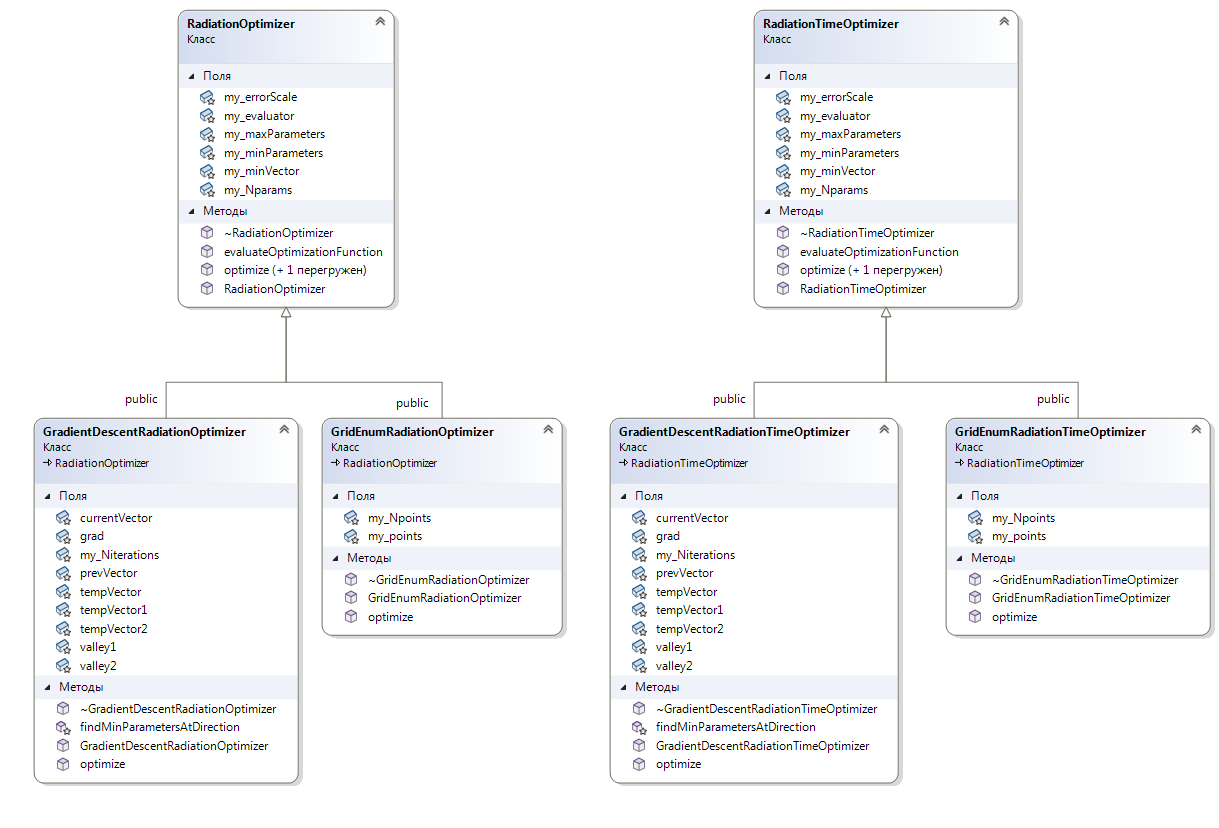
\includegraphics[width=11.5 cm]{./fig/radiationOptimizer.png} 
	\caption{Схема наследования классов оптимизаторов}
	\label{radiationOptimizer}
\end{figure}

\begin{small}
	\topcaption{Публичные методы классов оптимизаторов параметров источников }
	\label{RadiationOptimizerMethods}
	\begin{xtabular}{|p{0.41\textwidth}|p{0.59\textwidth}|}
		\hline
		\textbf{RadiationOptimizer} & абстрактный класс для оптимизации параметров источника \\
		\hline
		evaluateOptimizationFunction( const double* vector, double* energy, double* observedFlux, double* observedError, int Ne, RadiationSource* source) & вычисляет целевую функцию - взвешенную сумму квадратов ошибок во всех наблюдательных точках $f = \sum \frac{(F_i - F_{obs,i})^2}{\sigma_i^2}$, где $F_i$ - расчетная спектральная плотность потока излучения, $F_{obs,i}$ - наблюдаемая спектральная плотность потока излучения, $\sigma_i$ - её погрешность\\
		\hline
		optimize( double* vector, bool* optPar, double* energy, double* observedFlux, double* observedError, int Ne, RadiationSource* source) & функция, осуществляющая оптимизацию, принимает на вход массив подбираемых параметров, в который будет записан результат, массив булевских переменных, определяющих оптимизировать соответствующий параметр, или считать его фиксированным, массив энергий, на которых производились наблюдения, соответствующие наблюдаемые потоки в единицах $\text{см}^{-2}\text{с}^{-1}$, погрешности измерения потоков, количество наблюдательных точек, и источник излучения.\\
		\hline
		optimize( double* vector, bool* optPar, double* energy, double* observedFlux, int Ne, RadiationSource* source) & функция, осуществляющая оптимизацию, в случае не заданных наблюдательных ошибок. В таком случае ошибки у всех точек считаются равными елинице и веса всех ошибок в целевой функции оказываются равными\\
		\hline
		\textbf{GridEnumRadiationOptimizer} & класс предназначенный для оптимизации параметров с помощью перебора по сетке\\
		\hline
		GridEnumRadiationOptimizer( RadiationEvaluator* evaluator, const double* minParameters, const double* maxParameters, int Nparams, const int* Npoints) & конструктор, создает экземпляр класса с указанным вычислителем излучения, минимальными и максимальными значениями оптимизируемых параметров, количеством этих параметров и массивом с количеством перебираемых точек по каждому параметру. При переборе точки будут распределены логарифмически равномерно по оси.\\
		\hline
		\textbf{GradientDescentRadiationOptimizer} & класс, предназначенный для оптимизации параметров методом градиентного спуска\\
		\hline
		GradientDescentRadiationOptimizer( RadiationEvaluator* evaluator, const double* minParameters, const double* maxParameters, int Nparams, int Niterations) & конструктор, создает экземпляр класса с указанным вычислителем излучения, минимальными и максимальными значеними оптимизируемых параметров, количеством этих параметров и максимальным количеством итераций градиентного спуска\\
		\hline		
	\end{xtabular}
\end{small}

Пример фитирования параметров источника по наблюдательным данным приведен в функции fitCSS161010withPowerLawDistribition в файле examples.cpp. Следуя авторам работы \cite{Coppejans2020} произведем расчет синхротронного излучения источника с учетом самопоглощения, считая функцию распределения электронов чисто степенной с показателем 3.6. Но мы не будем накладывать дополнительную связь на параметры и предполагать равенство распределения энергии между магнитным полем и ускоренными частицами, вместо этого магнитное поле и концентрация электронов будут независимыми параметрами.

Подберем параметры Быстрого Оптического Голубого Транзиента CSS161010 на 98 день после вспышки на основе радиоизлучения. Зададим параметры источника на основе дынных статьи \cite{Coppejans2020}, которые будут использоваться в качестве начального приближения, а так же расстояние до него.
\begin{lstlisting}[language=c++]
    double electronConcentration = 25;
    double B = 0.6;
    double R = 1.4E17;
    double fraction = 0.5;
    const double distance = 150 * 1E6 * parsec;
\end{lstlisting}
Далее зададим степенное распределение электронов, с показателем 3.6 и источник в форме плоского диска, перпендикулярного лучу зрения, и вычислитель синхротронного излучения.
\begin{lstlisting}[language=c++]
    double Emin = me_c2;
    double Emax = 10000 * me_c2;
    double index = 3.6;
	
    SynchrotronEvaluator* synchrotronEvaluator = new 
	    SynchrotronEvaluator(200, Emin, Emax);
    MassiveParticlePowerLawDistribution* electrons = new 
	    MassiveParticlePowerLawDistribution(massElectron, index, 
	    Emin, electronConcentration);
    SimpleFlatSource* source = new 
	    SimpleFlatSource(electrons, B, 1.0, R, fraction*R, distance);
\end{lstlisting}
Теперь определим вектор оптимизируемых параметров - это размер, магнитное поле, концентрация электронов и доля толщины, показывающая какю долю от радиуса диска составляет его толщина. И именно такие параметры ожидает функция resetParameters у источника SimpleFlatSource. Так же нужно указать минимальные и максимальные значения параметров, которые ограничат область поиска. Максимальные значения так же будут использоваться как константы нормировки.
\begin{lstlisting}[language=c++]
    const int Nparams = 4;
    double minParameters[Nparams] = { 1E17, 0.01, 0.5, 0.1 };
    double maxParameters[Nparams] = { 2E17, 10, 200, 1.0 };
    double vector[Nparams] = { R, B, electronConcentration, fraction};
    for (int i = 0; i < Nparams; ++i) {
	    vector[i] = vector[i] / maxParameters[i];
    }
\end{lstlisting}
Зададим наблюдательные данные, которые и будем фитировать. Обратите внимание, что частоты нужно перевести в энергии, а спектральную плотность потока - в энергетическую (в единицы $\text{см}^{-2}\text{с}^{-1}$).
\begin{lstlisting}[language=c++]
    const int Nenergy1 = 4;
    double energy1[Nenergy1] = { 1.5E9*hplank, 3.0E9 * hplank, 
    	6.1E9 * hplank, 9.8E9 * hplank };
    double observedFlux[Nenergy1] = { 1.5/(hplank*1E26), 
    	4.3/(hplank*1E26), 6.1/(hplank*1E26), 4.2 /(hplank*1E26)};
    double observedError[Nenergy1] = { 0.1 / (hplank * 1E26), 
    	0.2/(hplank*1E26), 0.3/(hplank*1E26), 0.2/(hplank*1E26)};
\end{lstlisting}
Далее создадим два оптимизатора - действющий перебором и градиентым спуском, и применим их последовательно. Так же укажем количество точек для перебора и то, что оптимизируем все параметры.
\begin{lstlisting}[language=c++]
    bool optPar[Nparams] = { true, true, true, true };
    int Niterations = 20;
    int Npoints[Nparams] = { 10,10,10,10 };
    
    RadiationOptimizer* enumOptimizer = new GridEnumRadiationOptimizer(
        synchrotronEvaluator,minParameters,maxParameters,Nparams,Npoints);
    RadiationOptimizer* gradientOptimizer = new 
        GradientDescentRadiationOptimizer(synchrotronEvaluator, 
        minParameters, maxParameters, Nparams, Niterations);
\end{lstlisting}
Применим функцию optimize у последовательно у обоих оптимизаторов. Сначала перебором найдем начальное приближение, потом уточним результат с помощью градиентного спуска, и изменим параметры источника на оптимальные
\begin{lstlisting}[language=c++]
    enumOptimizer->optimize(vector, optPar, energy1, observedFlux, 
        observedError, Nenergy1, source);
    gradientOptimizer->optimize(vector, optPar, energy1, observedFlux, 
        observedError, Nenergy1, source);
    source->resetParameters(vector, maxParameters);
\end{lstlisting}
Полученные в результате оптимизации парметры источника равны: радиус диска $R = 1.8\times10^17 \text{ см}$, магнитное поле $B = 1.6 \text{ Гс}$, концентрация электронов $n = 2.3 \text{ см}^{-3}$, доля толщины $fraction = 0.54 $. Значение целевой функции $f \approx 50$. Модельный спектр излучения  с данными параметрами и наблюдательные данные изображены на рисунке \ref{synchrotron1}.
\begin{figure}
	\centering
	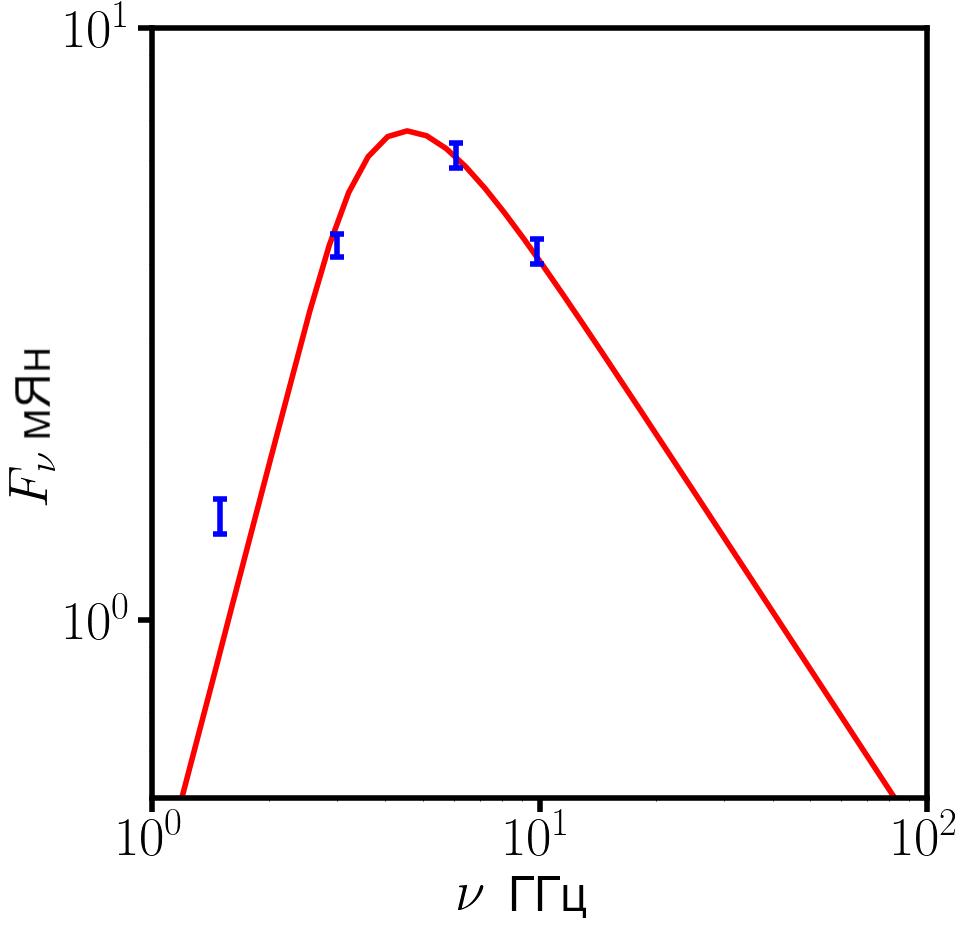
\includegraphics[width=12.5 cm]{./fig/synchrotron1.png} 
	\caption{Наблюдаемый и расчетный спектр радиоизлучения объекта CSS161010 на 98 день после вспышки}
	\label{synchrotron1}
\end{figure}
\section{Фитирование источников, зависящих от времени}
Для фитирования постоянных во времени кривых блеска изменяющихся во времени предназначен абстрактный класс RadiationTimeOptimizer. В нем определена виртуальныя функция optimize(double* vector, bool* optPar, double** energy, double** observedFLux, double** observedError, int* Ne, int Ntimes, double* times, RadiationTimeDependentSource* source), которая и выполняет оптимизацию. Так же как и в случае не зависящей от времени оптимизации она принимает на вход массив параметров, массив булевских переменных, и наблюдательные данные. Но наблюдательные данные теперь представляют собой двумерные массивы (причем количество заданных точек в разные моменты времени так же может быть разным). Так же нужно указать количество серий измерений во времени и соответствующие им времена. Исследуемый источник должен относиться к классу зависящих от времени источников.

Как и ранее, в коде реализованы два наследника класса RadiationTimeOptimazer: GridEnumRadiationTimeOptimizer - для поиска минимума перебором, и GradientDescentRadiationTimeOptimizer - в котором минимум находится методом градиентного спуска. Схема насследования классов оптимизаторов показана на рисунке \ref{radiationOptimizerTime}, а список их публичных методов приведен в Таблице \ref{RadiationTimeOptimizerMethods}.
\begin{figure}
	\centering
	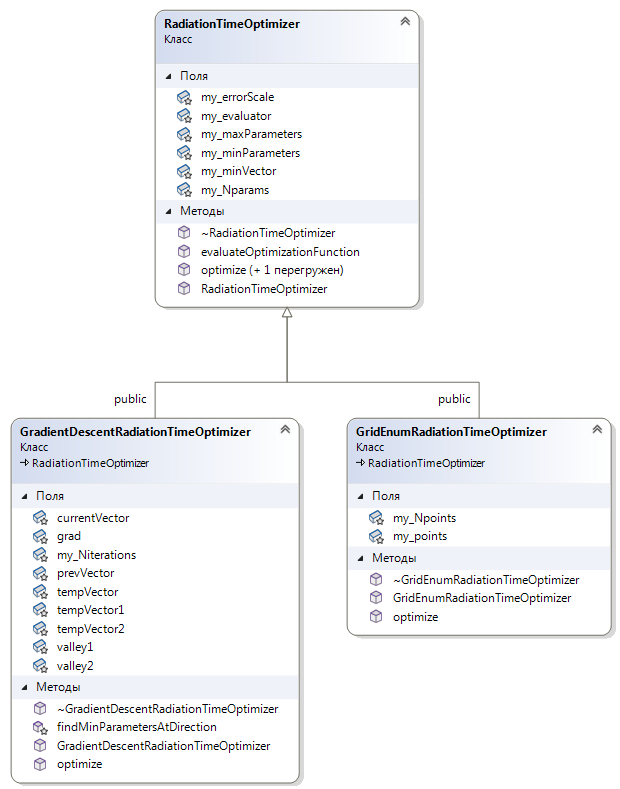
\includegraphics[width=10.5 cm]{./fig/radiationOptimizerTime.png} 
	\caption{Схема наследования классов оптимизаторов, учитывающих переменность источников}
	\label{radiationOptimizerTime}
\end{figure}

\begin{small}
	\topcaption{Публичные методы классов оптимизаторов параметров переменных во времени источников }
	\label{RadiationTimeOptimizerMethods}
	\begin{xtabular}{|p{0.5\textwidth}|p{0.5\textwidth}|}
		\hline
		\textbf{RadiationTimeOptimizer} & абстрактный класс, предназначенный для оптимизации параметров зависящих от времени источников\\
		\hline
		evaluateOptimizationFunction( const double* vector, double** energy, double** observedFlux, double** observedError, int* Ne, int Ntimes, double* times, RadiationTimeDependentSource* source) & вычисляет целевую функцию - взвешенную сумму квадратов ошибок во всех наблюдательных точках во все моменты времени $f = \sum \frac{(F_i - F_{obs,i})^2}{\sigma_i^2}$, где $F_i$ - расчетная спектральная плотность потока излучения, $F_{obs,i}$ - наблюдаемая спектральная плотность потока излучения, $\sigma_i$ - её погрешность\\
		\hline
		optimize (double* vector, bool* optPar, double** energy, double** observedFLux, double** observedError, int* Ne, int Ntimes, double* times, RadiationTimeDependentSource* source) & функция, осуществляющая оптимизацию, принимает на вход массив подбираемых параметров, в который будет записан результат, массив булевских переменных, определяющих оптимизировать соответствующий параметр, или считать его фиксированным, двумерные массивы энергий, на которых производились наблюдения, соответствующих энергиям наблюдаемых потоков в единицах $\text{см}^{-2}\text{с}^{-1}$, погрешности наблюдаемых потоков, массив количества наблюдательных точек в каждый момент времени, количество моментов времени, когда производились измерения, соответствующие времена и переменный источник излучения.\\
		\hline
		optimize(double* vector, bool* optPar, double** energy, double** observedFlux, int* Ne, int Ntimes, double* times, RadiationTimeDependentSource* source) & функция, осуществляющая оптимизацию, в случае не заданных наблюдательных ошибок. В таком случае ошибки у всех точек считаются равными елинице и веса всех ошибок в целевой функции оказываются равными\\
		\hline
		\textbf{GridEnumRadiationTimeOptimizer} & класс, предназначенный для оптимизации параметров переменных источников с помощью перебора по сетке\\
		\hline
		GridEnumRadiationTimeOptimizer( RadiationEvaluator* evaluator, const double* minParameters, const double* maxParameters, int Nparams, const int* Npoints) & конструктор, создает экземпляр класса с указанным вычислителем излучения, минимальными и максимальными значениями оптимизируемых параметров, количеством этих параметров и массивом с количеством перебираемых точек по каждому параметру. При переборе точки будут распределены логарифмически равномерно.\\
		\hline
		\textbf{GradientDescentRadiationTimeOptimizer} & класс, предназначенный для оптимизации параметров переменных источников методом градиентного спуска\\
		\hline
		GradientDescentRadiationTimeOptimizer( RadiationEvaluator* evaluator, const double* minParameters, const double* maxParameters, int Nparams, int Niterations) & конструктор, создает экземпляр класса с указанным вычислителем излучения, минимальными и максимальными значеними оптимизируемых параметров, количеством этих параметров и максимальным количеством итераций градиентного спуска\\
		\hline		
\end{xtabular}
\end{small}

Пример фитирования параметров источника по наблюдательным данным приведен в функции fitTimeDependentCSS161010() в файле examples.cpp. Подберем параметры Быстрого Оптического Голубого Транзиента CSS161010 на основе наблюдений радиоизлучения, проведенных на 98, 162, 357 день после вспышки.  Расчет синхротронного излучения учитывает самопоглощение и раширение источника. Источник будем считать шаровым слоем с однородной плотностью и однороным магнитным полем, направленным перпендикулярно лучу зрения. Функцию распределения излучающих электронов возьмем на основе Particle-in-Cell расчетов для ударной волны со скоростью 0.3c,как сделано в работе \cite{BykovUniverse}. Учтена зависимость функции распределения от угла между магнитным полем и направлением распространения ударной волны.

Подберем параметры Быстрого Оптического Голубого Транзиента CSS161010 на основе наблюдений радиоизлучения, проведенных на 98, 162, 357 день после вспышки. 
\begin{lstlisting}[language=c++]
double electronConcentration = 25;
double B = 0.6;
double R = 1.4E17;
double fraction = 0.5;
const double distance = 150 * 1E6 * parsec;
\end{lstlisting}
			% Глава 2. Оптимизация параметров
%\chapter{Формулы расчета излучения}\label{Formulae}

\section{Преобразование функции распределения фотонов}
Функция распределения фотонов задана в сферических координатах $n_{ph}(\epsilon,\mu,\phi)$. Рассмотрим переход в систему отсчета, движущуюся в направлении оси $z$ с лоренц-фактором $\gamma = 1/\sqrt{1-\beta^2}$. Количество частиц в элементе фазового пространства $N$ - инвариант.
\begin{equation}
	N = n_{ph}(\epsilon,\mu,\phi)d\epsilon d\mu d\phi dV = n'_{ph}(\epsilon',\mu',\phi')d\epsilon' d\mu' d\phi' dV'
\end{equation}
Рассмотрим преобразование вектора четырех-импульса. Поперечные компоненты не изменяются, а временная и продольная меняются следющим образом, учитывая что $p_z = \mu \epsilon$:
\begin{equation}\label{lorentz_ph}
	\left(\begin{array}{c}
		\epsilon'\\
		\mu'\epsilon'
	\end{array}
	\right)
	= \left(
	\begin{array}{cc}
		\gamma & -\beta\gamma\\
		-\beta\gamma & \gamma
	\end{array}
	\right)
	\times
	\left(\begin{array}{c}
		\epsilon\\
		\mu\epsilon
	\end{array}
	\right)
\end{equation}
Из первой строчки матрицы получаем уравнение для допплеровского сдвига энергии
\begin{equation}\label{doppler_ph}
	\epsilon'=\gamma(1-\mu\beta)\epsilon
\end{equation}
Вычислим производные новой энергии по старым координатам
\begin{equation}
	\frac{d\epsilon'}{d\epsilon}=\gamma(1-\mu\beta)
\end{equation}
\begin{equation}
	\frac{d\epsilon'}{d\mu}=-\gamma\beta\epsilon
\end{equation}
Из второй строчки матрицы получаем $\mu'\epsilon'=-\beta\gamma\epsilon+\gamma\mu\epsilon$. Подставив значение $\epsilon'$ из \ref{doppler_ph} и сократив $\epsilon$ получим уравнение аберрации света
\begin{equation}\label{aberration_ph}
	\mu'=\frac{\mu-\beta}{1-\mu\beta}
\end{equation}
Заметим, что угол наклона луча в новой системе не зависит от энергии в старой системе. Вычислим частноую производную $\frac{d\mu'}{d\mu}$
\begin{equation}
	\frac{d\mu'}{d\mu}=\frac{d}{d\mu}\frac{1}{\beta}\frac{\beta\mu-1+1-\beta^2}{1-\mu\beta}=\frac{d}{d\mu}\frac{1}{\beta}\frac{1-\beta^2}{1-\mu\beta}=\frac{1-\beta^2}{(1-\mu\beta)^2}=\frac{1}{\gamma^2(1-\mu\beta)^2}
\end{equation}
Азимутальный угол не зависит от системы отсчета $\phi' = \phi$. Преобразование элемента объема описывается выражением $\frac{dV'}{dV} = \frac{\epsilon}{\epsilon'}$ см. ЛЛ Т2 параграф 10, вот только там используется переход в собственную систему. То есть
\begin{equation}
	\frac{dV'}{dV} = \frac{1}{\gamma(1-\mu\beta)}
\end{equation}
Матрица якоби преобразования координат выглядит следующим образом
\begin{equation}
	J=\left(
	\begin{array}{cccc}
		\frac{d\epsilon'}{d\epsilon} & \frac{d\epsilon'}{d\mu}& 0 & 0\\
		0 & \frac{d\mu'}{d\mu} & 0 & 0\\
		0 & 0 & 1 & 0\\
		0 & \frac{dV'}{d\mu} & 0 & \frac{dV'}{dV}
	\end{array}
	\right)
\end{equation}
При такой матрице якобиан, к счастью, равен произведению диагональных членов
\begin{equation}\label{jacobian_ph}
	\frac{D(\epsilon',\mu',\phi',V')}{D(\epsilon,\mu,\phi,V)}=\frac{d\epsilon'}{d\epsilon}\frac{d\mu'}{d\mu}\frac{dV'}{dV}=\gamma(1-\mu\beta)\frac{1}{\gamma^2(1-\mu\beta)^2}\frac{1}{\gamma(1-\mu\beta)}=\frac{1}{\gamma^2(1-\mu\beta)^2}
\end{equation}
И в итоге функция распределения фотонов преобразуется с помощью деления на вычисленный якобиан
\begin{equation}\label{distribution_ph}
	n'_{ph}(\epsilon',\mu',\phi') = \frac{n_{ph}(\epsilon,\mu,\phi)}{\frac{D(\epsilon',\mu',\phi',V')}{D(\epsilon,\mu,\phi,V)}}=\gamma^2(1-\mu\beta)^2 n_{ph}(\epsilon,\mu,\phi)
\end{equation}
\section{Комптоновское рассеяние}
Рассмотрим рассеяние фотонов на одном электроне, движущемся вдоль ось z, см \cite{Dubus}. Сечение Клейна-Нишины в системе покоя электрона равно
\begin{equation}
	\frac{d\sigma}{d\epsilon_1'd\Omega_1'}=\frac{{r_e}^2}{2}\left(\frac{\epsilon_1'}{\epsilon_0'}\right)^2(\frac{\epsilon_1'}{\epsilon_0'}+\frac{\epsilon_0'}{\epsilon_1'}-\sin^2\Theta') \delta(\epsilon_1' - \frac{\epsilon_0'}{1+\frac{\epsilon_0'}{m_e c^2}(1 - \cos \Theta')})
\end{equation}
Где $r_e$ - классический радиус электрона, $\epsilon_0'$ и $\epsilon_1'$ - энергии начального и конечного фотона, соответственно, $\Theta'$ - угол между начальным и конечным фотоном, определяемый выражением $\cos\Theta' =\cos \theta_0' \cos \theta_1' + \sin \theta_0' \sin \theta_1' \cos(\phi_1' - \phi_0')$. Штрихованные индексы относятся к системе отсчета электрона. При этом начальная и конечная энергии фотонов оказываются связаны соотношениями
\begin{equation}
	\epsilon_1'=\frac{\epsilon_0'}{1+\frac{\epsilon_0'}{m_e c^2}(1 - \cos \Theta')}	
\end{equation}
\begin{equation}
	\epsilon_0'=\frac{\epsilon_1'}{1-\frac{\epsilon_1'}{m_e c^2}(1 - \cos \Theta')}
\end{equation}
Число фотонов, рассеявшихся в заданный телесный угол в единицу времени в промежуток энергии в системе покоя электрона равно
\begin{equation}
\frac{dN'}{dt'd\epsilon_1'd\Omega_1'}=\int c \frac{d\sigma}{d\epsilon_1'd\Omega_1'} \frac{dn'}{d\epsilon_0'd\Omega_0'}d\Omega_0'd\epsilon_0'
\end{equation}

Перепишем дельта-функцию через энергию начального фотона с помощью соотношения 
\begin{equation}
	\delta(f(x)) = \sum \frac{\delta(x-x_k)}{|f'(x_k)|}
\end{equation}
где $x_k$ - корни функции $f(x)$. Производная выражения внутри дельта-функции равна
\begin{equation}
	\frac{d\epsilon_1'}{d\epsilon_0'}=\frac{1}{(1+\frac{\epsilon_0'}{m_e c^2}(1 - \cos \Theta'))^2}
\end{equation}
и она сократится с квадратом отношения энергий в формуле для сечения. Функцию распределения начальных фотонов выразим в лабораторной системе с помощью выражения \ref{distribution_ph}.
\begin{equation}
	\frac{dN'}{dt'd\epsilon_1'd\Omega_1'}=\int \frac{r_e^2 c}{2} \gamma_e^2 (1 - \mu_0 \beta_e)^2 (\frac{\epsilon_1'}{\epsilon_0'}+\frac{\epsilon_0'}{\epsilon_1'}-\sin^2\Theta')\frac{dn}{d\epsilon_0 d\Omega_0} \delta(\epsilon_0' - \frac{\epsilon_1'}{1-\frac{\epsilon_1'}{m_e c^2}(1 - \cos \Theta')}) d\epsilon_0'd\mu_0' d\phi_0'
\end{equation}
Теперь избавимся от дельта-функции, проинтегрировав по $\epsilon_0'$.
\begin{equation}
	\frac{dN'}{dt'd\epsilon_1'd\Omega_1'}=\int \frac{r_e^2 c}{2} \gamma_e^2 (1 - \mu_0 \beta_e)^2 (1 + \cos^2\Theta'+(\frac{\epsilon_1'}{m_e c^2})^2\frac{(1-\cos\Theta')^2}{1-\frac{\epsilon_1'}{m_e c^2}(1 - \cos \Theta')})\frac{dn}{d\epsilon_0 d\Omega_0}d\mu_0' d\phi_0'
\end{equation}
Осталось перевести поток рассеяных фотонов в лабораторную систему отсчета $\frac{dN}{dt d\epsilon_1 d\Omega_1} = \frac{dN'}{dt' d\epsilon_1' d\Omega_1'}\frac{dt'}{dt}\frac{d\epsilon_1'}{d\epsilon_1}\frac{d\Omega_1'}{d\Omega_1}$. Используя то, что $dt = \gamma_e dt'$, $\epsilon = \frac{1}{\gamma_e(1 -\mu_1\beta_e)}\epsilon'$ и $\mu_1' = \frac{\mu_1-\beta_e}{1-\mu_1 \beta_e}$ получим
\begin{equation} \label{compton_elframe}
	\frac{dN}{dt d\epsilon_1 d\Omega_1}=\int \frac{r_e^2 c}{2} \frac{(1 - \mu_0 \beta_e)^2}{1-\mu_1\beta_e} (1 + \cos^2\Theta'+(\frac{\epsilon_1'}{m_e c^2})^2\frac{(1-\cos\Theta')^2}{1-\frac{\epsilon_1'}{m_e c^2}(1 - \cos \Theta')})\frac{dn}{d\epsilon_0 d\Omega_0}d\mu_0' d\phi_0'	
\end{equation}
При интегрировании нужно выразить углы в лабораторной системе отсчета $\mu_0, \phi_0$ через переменные интегрирования $\mu_0', \phi_0'$. Для расчета рассеяния на распределении электронов нужно проинтегрировать формулу \ref{compton_elframe} с функцией распределения электронов, нормированной на количество частиц. При этом надо учесть разные направления движения электронов и произвести повороты углов.

Так же может быть удобно интегрировать в переменных лабораторной системы расчета, тогда выражение для потока фотонов будет следующим
\begin{equation}\label{compton_labframe}
	\frac{dN}{dt d\epsilon_1 d\Omega_1}=\int \frac{r_e^2 c}{2} \frac{1}{\gamma_e^2(1-\mu_1\beta_e)} (1 + \cos^2\Theta'+(\frac{\epsilon_1'}{m_e c^2})^2\frac{(1-\cos\Theta')^2}{1-\frac{\epsilon_1'}{m_e c^2}(1 - \cos \Theta')})\frac{dn}{d\epsilon_0 d\Omega_0}d\mu_0 d\phi_0
\end{equation}
При рассмотрении процессов, связанных с электронами высоких энергий $\gamma_e \approx 10^8$ относительные численные погрешности вычислений могут быть очень велики, так как $\beta_e$ и $\mu_0, \mu_1, \cos \Theta'$ оказываются слишком близки к единице и стандартный тип double может не разрешать это отличие. Поэтому для численных вычислений оказывается полезным ввести следующие вспомогательные величины:
\begin{equation}
	\delta_e = 1 - \beta_e
\end{equation}
\begin{equation}
	\text{versin}~\theta = 1 - \cos \theta
\end{equation}
Тогда выражения вида $1 - \mu \beta_e$ в этих величинах перепишется как
\begin{equation}
	1 - \mu \beta_e =\text{versin}~\theta + \delta_e - \text{versin}~\theta~\delta_e
\end{equation}
а выражение для угла между конечным и начальным фотоном как
\begin{equation}
	1 - \cos \Theta' = \text{versin}~\theta_0' + \text{versin}~\theta_1' - \text{versin}~ \theta_0' \text{versin}~\theta_1' - \sin \theta_0'\sin \theta_1' \cos(\phi_1'-\phi_0')
\end{equation}
С использованием данных выражений значительно повышается точность и максимальные доступные к рассмотрению энергии фотонов и электронов.

В случае изотропных функций распределения фотонов и релятивистских электронов можно произвести аналитическое интегрирование по угловым переменным \cite{JonesCompton, BykovUvarov2000}, и тогда для вычисления излучения достаточно лишь провести интегрирования по энергиям по формуле
\begin{equation}
	\frac{dN}{dt d\epsilon_1 d\Omega_1}=\int \frac{2 \pi r_e^2 m_e c^3 }{\epsilon_0 \gamma_e^2} \frac{dn_{ph}}{d\epsilon_0}\frac{dn_e}{d\epsilon_e}(2 q~ \ln(q)+1+q-2q^2+\frac{q^2(1-q)\Gamma^2}{2(1+q\Gamma)})d\epsilon_0d\epsilon_e
\end{equation}
где $\Gamma=4\epsilon_0\gamma_e/m_e c^2$, $q=\epsilon_1/((\gamma_e m_e c^2-\epsilon_1)\Gamma)$.
\section{Синхротронное излучение}
Процесс синхротронного излучения хороши известен и описан в классических работах. Но с точки зрения квантовой электродинамки, любому процессу излучения можно так же сопоставить процесс поглощения. Сечение процесса синхротронного самопоглощения описано в работе Гизеллини и Свенсона \cite{Ghisellini1991}. Спектральная плотность мощности излучения единицы объема вещества определеяется формулой
\begin{equation} \label{emission}
	I(\nu)=\int_{E_{min}}^{E_{max}} dE \frac {\sqrt {3}{e}^{3}n F(E) B \sin ( \phi)}{{m_e}{c}^{2}}
	\frac{\nu}{\nu_c}\int_{\frac {\nu}{\nu_c}}^{\infty }\it K_{5/3}(x)dx,
\end{equation}
где $\phi$ это угол межде вектором магнитного поля и лучом зрения, $\displaystyle\nu_{c}$ критическая частота, определяемая выражением $\displaystyle\nu_{c} = 3 e^{2} B \sin(\phi) E^{2}/4\pi {m_{e}}^{3} c^{5}$, и~$K_{5/3}$ - функция МакДональда.
Коэффициент поглощения для фотонов, распростроняющихся вдоль луча зрения равен
\begin{equation}\label{absorption}
	k(\nu)=\int_{E_{min}}^{E_{max}}dE\frac {\sqrt {3}{e}^{3}}{8\pi m_e \nu^2}\frac{n B\sin(\phi)}{E^2}
	\frac{d}{dE} E^2 F(E)\frac {\nu}{ \nu_c}\int_{\frac {\nu}{ \nu_c}}^{\infty }K_{5/3}(x) dx.
\end{equation}			% Глава 3. Формулы расчета излучения
%\addcontentsline{toc}{chapter}{\bibname}	% Добавляем список литературы в оглавление
\linespread{1}\selectfont
%\bibliography{introduction,part1,part2,part3,part4,part5}
\bibliography{part1}  
%\bibliography{part2}  
%\bibliography{part3} 
%\bibliography{part4} 
% Подключаем BibTeX-базы
		% Список литературы
%\input{appendix}     % Приложения

\end{document}
